%% ---------------------------------------------------------------------------
%%  SINGLE-COLUMN version  (this is the file to compile if you want the paper
%%  in one column: full-width text, single spacing, IEEE typography)
%%
%%  The manuscript body is the shared file body.tex, so the text, numbering,
%%  figures, tables and references are identical to the two-column version.
%%
%%  Build:  pdflatex main_singlecolumn && bibtex main_singlecolumn &&
%%          pdflatex main_singlecolumn && pdflatex main_singlecolumn
%%
%%  Layout choices:
%%    * one column, A4, 2.5 cm margins, 11 pt Times (mathptmx)
%%    * IEEE-style headings:  I. INTRODUCTION  (centred, small capitals),
%%      A. Subsection  (italic, flush left)
%%    * IEEE-style abstract and Index Terms paragraphs
%%    * appendices numbered A, B (Appendix A, Appendix B)
%%  No IEEEtran.cls is needed, so this file compiles anywhere, including a
%%  minimal TeX installation.
%% ---------------------------------------------------------------------------
\documentclass[11pt,a4paper]{article}

\usepackage[T1]{fontenc}
\usepackage[utf8]{inputenc}
\usepackage{lmodern}          % fallback; mathptmx below sets Times
\usepackage{mathptmx}         % Times text and Times-based math
\usepackage[margin=2.5cm]{geometry}
\usepackage{amsmath,amssymb,amsthm,mathtools}
\usepackage{mathrsfs}
\usepackage{graphicx}
\usepackage{booktabs,array,tabularx}
\usepackage[font=small,labelfont=bf,justification=centering]{caption}
\usepackage{url}
\usepackage{microtype}
\usepackage[hidelinks]{hyperref}

\graphicspath{{figures/}}

% ---------------------------------------------------------------------------
% IEEE-style section headings with Roman numerals
% ---------------------------------------------------------------------------
\makeatletter
\renewcommand\thesection{\Roman{section}}
\renewcommand\thesubsection{\thesection-\Alph{subsection}}% not used visually
\renewcommand\section{\@startsection{section}{1}{\z@}%
  {-3.5ex \@plus -1ex \@minus -.2ex}%
  {2.3ex \@plus .2ex}%
  {\normalfont\normalsize\scshape\centering}}
\renewcommand\subsection{\@startsection{subsection}{2}{\z@}%
  {-3.25ex\@plus -1ex \@minus -.2ex}%
  {1.5ex \@plus .2ex}%
  {\normalfont\normalsize\itshape}}
\renewcommand\subsubsection{\@startsection{subsubsection}{3}{\z@}%
  {-3.25ex\@plus -1ex \@minus -.2ex}%
  {1.5ex \@plus .2ex}%
  {\normalfont\normalsize\itshape}}
% subsection labels as "A.", "B.", ... (IEEE style)
\renewcommand\thesubsection{\Alph{subsection}}
\makeatother

% IEEE-style appendix: \appendices switches to A, B, ... sections
\newcommand{\appendices}{%
  \par\appendix
  \setcounter{section}{0}%
  \renewcommand{\thesection}{\Alph{section}}%
  \renewcommand{\thesubsection}{\thesection.\arabic{subsection}}%
}

% ---------------------------------------------------------------------------
% theorem environments, numbered consecutively as in IEEE journals
% ---------------------------------------------------------------------------
\theoremstyle{plain}
\newtheorem{theorem}{Theorem}
\newtheorem{lemma}[theorem]{Lemma}
\newtheorem{proposition}[theorem]{Proposition}
\newtheorem{corollary}[theorem]{Corollary}
\theoremstyle{definition}
\newtheorem{definition}[theorem]{Definition}
\newtheorem{example}[theorem]{Example}
\theoremstyle{remark}
\newtheorem{remark}[theorem]{Remark}

% ---------------------------------------------------------------------------
% macros shared with body.tex
% ---------------------------------------------------------------------------
\newcommand{\F}{\mathbb F}
\newcommand{\K}{\mathbb K}
\newcommand{\A}{\mathcal A}
\newcommand{\Fs}{\mathcal F_s}
\newcommand{\Os}{\mathcal O_s}
\newcommand{\Epoly}{\mathscr E}
\newcommand{\Hull}{\operatorname{Hull}}
\newcommand{\rank}{\operatorname{rank}}
\newcommand{\Dk}{D_k}
\newcommand{\perpE}{\perp_{E}}
\newcommand{\Frob}{\operatorname{Frob}}
\newcommand{\lcm}{\operatorname{lcm}}

\setlength{\parindent}{1.5em}
\setlength{\parskip}{0pt}

\begin{document}

\title{\bfseries Joint Code-Dimension and \texorpdfstring{$k$}{k}-Galois-Hull
Enumerators for Repeated-Root Constacyclic Codes over Square-Free Affine
Algebras}

\author{Arun Kumar Yadav\textsuperscript{1}, Vipin Gupta\textsuperscript{2},
Pooja Soni\textsuperscript{3}, and Manju Pruthi\textsuperscript{4}%
\thanks{Manuscript received XXXX XX, 2026; revised XXXX XX, 2026; accepted
XXXX XX, 2026. This work received no external funding. (Corresponding author:
Arun Kumar Yadav.)}%
\thanks{\textsuperscript{1}A. K. Yadav is with the School of Basic and Applied
Sciences, K.R. Mangalam University, Sohna Road, Gurugram 122103, Haryana, India
(e-mail: arunyadav0307@gmail.com; ORCID iD: 0009-0009-1169-3264).}%
\thanks{\textsuperscript{2}V. Gupta is with the Department of Mathematics,
Gurugram University, Sector 51, Gurugram 122003, Haryana, India
(e-mail: \texttt{XXXX}).}%
\thanks{\textsuperscript{3}P. Soni is with the Department of Mathematics,
Lovely Professional University, Jalandhar--Delhi G.T. Road, Phagwara 144411,
Punjab, India (e-mail: \texttt{XXXX}).}%
\thanks{\textsuperscript{4}M. Pruthi is with the Department of Mathematics,
Indira Gandhi University, Meerpur, Rewari 122502, Haryana, India
(e-mail: \texttt{XXXX}).}%
\thanks{Digital Object Identifier 10.1109/TIT.2026.XXXXXXX (to appear).}%
\thanks{Supplementary material: the Python implementation of the enumerator and
the complete verification log described in the section on computational
verification are included with the submission.}}

\date{}

\maketitle
\thispagestyle{empty}

\vspace{-1.2em}

\noindent\textbf{\textit{Abstract}}---We determine the exact joint distribution
of the code dimension and the $k$-Galois hull dimension over all repeated-root
constacyclic codes of a fixed length over a square-free affine algebra over a
finite field. With length $n=n'p^{t}$ and component moduli that are $p^{t}$-th
powers of square-free kernels, a code is encoded by one exponent at each
distinct kernel factor, and the $k$-Galois dual acts on those factors through a
Frobenius-twisted reciprocal permutation. On each orbit of this permutation the
hull dimension is a cyclic sum of pairwise minima of consecutive exponents, so
its bivariate law is the trace of a power of an explicit weighted transfer
matrix with $p^{t}+1$ states; multiplying over orbits, with a dimension-only
factor for components whose twist is incompatible, gives a bivariate polynomial
whose coefficients are the exact multiplicities of the pairs (code dimension,
hull dimension). We obtain the marginal laws, the attainable pairs, closed
means and variances, conditional laws, and the numbers of LCD,
self-orthogonal, dual-containing and self-dual codes, and we give an algorithm
that is polynomial in the length, the multiplicity and the number of kernel
factors, checked against finite-field computations in characteristics $2$, $3$
and $5$.

\vspace{0.4em}
\noindent\textbf{\textit{Index Terms}}---Constacyclic codes, Galois hulls, LCD
codes, repeated-root codes, transfer matrices.

\vspace{0.4em}
\noindent\rule{\textwidth}{0.4pt}

\section{Introduction}\label{sec:intro}
The hull of a linear code $C$ is the intersection of $C$ with its dual.
Codes with trivial hull are the linear complementary dual (LCD) codes
introduced by Massey \cite{massey1992}, which meet the Gilbert--Varshamov
bound \cite{sendrier2004}; for cyclic codes a simple root condition
characterizes them \cite{yangMassey1994}. The hull dimension also enters exact
counts of linear codes \cite{sendrier1997}, and in the quantum setting it
determines the number of maximally entangled pairs required by
entanglement-assisted quantum codes \cite{brun2006,wildeBrun2008}, a
construction developed for cyclic and constacyclic families in
\cite{guendaJitmanGulliver2018}. The
$k$-Galois hull, introduced by Fan and Zhang \cite{fanZhang2017}, replaces
one slot of the coordinate pairing by a Frobenius power, unifying, at the
field level, the Euclidean and Hermitian cases; Galois self-orthogonal
constacyclic codes and MDS codes with Galois hulls of prescribed dimension are
treated in \cite{fuLiu2022} and \cite{cao2021}. For a constacyclic code, whose codewords are
represented by polynomials modulo $x^n-\lambda$, duals and hulls are again
ideals under suitable conditions, so factorization arguments apply
\cite{huffmanPless2003}.

Most Galois-hull results describe one code at a time. Liu and Pan
\cite{liuPan2020} compute Galois hull dimensions of general linear codes from
generator matrices. For constacyclic codes over finite fields, Debnath et
al.\ \cite{debnathConstacyclic2023} (see also the correction
\cite{debnathCorrection2023}) give a factor-theoretic hull-dimension
formula and, under restrictions on the field parameters, count the codes
with a prescribed hull dimension, extending the Euclidean and Hermitian
enumeration of Sangwisut et al.\ \cite{sangwisut2015}. At the level of
generator descriptions, Taki Eldin and Sol\'e \cite{eldinSole2026} obtain
generator polynomial matrices for Galois hulls of multi-twisted codes over
finite fields, and intersections of linear and multi-twisted codes are
described in \cite{eldinLeroy2026}. A parallel line studies averages rather than full
distributions: Skersys \cite{skersys2003} for cyclic codes over fields,
Jitman and Sangwisut \cite{jitmanSangwisut2018} for Hermitian hulls, and
Debnath and Prakash \cite{debnathAverage2025} for Galois hulls over finite
fields and over a finite non-chain ring; the attainability of small Galois
hull dimensions is studied in \cite{debnathSmall2026}, and the sequence of
numbers of linear codes with increasing hull dimension in
\cite{bouyuklieva2026}. Closest to the
algebraic setting of this paper, Debnath, Islam, Mart\'inez-Moro and Prakash
\cite{debnathAffine2026} study $k$-Galois hulls of constacyclic codes over
affine algebra rings: they describe dual and hull generators in idempotent
form, derive a hull-dimension formula for an individual code---under the
hypotheses $\gcd(\operatorname{ord}\lambda,n')=1$ and
$\operatorname{ord}\lambda\mid 1+p^{e-k}$---and give an LCD criterion and
quantum-code applications. In the repeated-root regime $p\mid n$ the
per-code hull-dimension formula is also known for constacyclic codes over a
single field \cite{debnathConstacyclic2023}, and we use it as a check rather
than a claim (Remark~\ref{rem:debnath-agreement}). None of these works
records how the pairs (code dimension, hull dimension) are distributed over
a whole family.

The present paper is concerned with \emph{repeated-root} lengths, that is,
with $p\mid n$ in characteristic $p$, where the modulus $x^n-\lambda$ is a
perfect power rather than a square-free polynomial. Repeated-root cyclic
codes were investigated in generality by Castagnoli, Massey, Schoeller and
von Seemann \cite{castagnoli1991} and by van Lint \cite{vanLint1991}, who
showed that such families are asymptotically bad; nevertheless their finite
algebraic structure---generators, duals and distances at specific
lengths---has been developed extensively, for example in
\cite{dinh2012}, in the study of constacyclic codes of prime-power length over
rings \cite{dinh2010}, and in the chain-ring theory of
\cite{dinhLopezPermouth2004}; see also \cite{nortonSalagean2000}. Within the hull theme,
Pang, Zhu and Li \cite{pangZhuLi2018} characterize and enumerate the LCD
repeated-root cyclic codes over a finite field, hulls of cyclic codes over $\mathbb{Z}_4$ are computed in
\cite{jitmanZ4}, and Fan and Zhang
\cite{fanZhang2017} treat Galois self-dual constacyclic codes over fields,
including repeated-root examples in characteristic $2$. What is missing is
the population-level picture for repeated-root lengths: the number of codes
with each code dimension and each $k$-Galois hull dimension.

For a repeated-root length, write $n=n'p^t$ with $\gcd(n',p)=1$ and put
$M=p^t$. Componentwise, the Frobenius identity writes the modulus as the
$M$-th power of a square-free kernel. A code is therefore determined by an
exponent in $\{0,\dots,M\}$ at each distinct irreducible factor of that
kernel. Along a compatible Frobenius-twisted reciprocal orbit, the hull
statistic is a cyclic sum of pairwise minima of these exponents
(Proposition~\ref{prop:min-edge}), and its bivariate law is encoded by an
$(M+1)$-state transfer matrix. The resulting formulas separate the variance
into three orbit-length regimes; length-$1$ orbits can contribute positive
hull dimension; and, for $t\geq1$ in characteristic $2$, self-dual codes can
arise through the midpoint exponent $M/2$
(Section~\ref{sec:consequences}).

We keep the coefficient algebra square-free, so that
$\A\cong\prod_s K_s$ with $K_s=\F_{p^{d_s}}$, and allow the length to be
arbitrary. All $\A$-linear $\lambda$-constacyclic codes of length $n=n'p^t$
are counted, as labeled submodules determined by the exponents of the
distinct irreducible factors of the square-free kernel $x^{n'}-\lambda_0$, and
all twists $\lambda\in\A^\ast$ are allowed: components whose twist is
incompatible with the $k$-Galois dual contribute hull dimension $0$ and are
included with an explicit dimension-only factor. The main result
(Theorem~\ref{thm:main}) is the exact joint enumerator
\begin{align*}
  \Epoly^{(M)}(U,Z)
  &=\sum_{C} U^{\kappa(C)} Z^{\eta_k(C)}\\
  &=\prod_{s\ \mathrm{compatible}}\prod_{O\in\Os}
     \operatorname{tr}\!\bigl((T^{(M)}_{w_O})^{a_O}\bigr)
   \prod_{s\ \mathrm{incompatible}}\prod_{f\in\Fs}
     \bigl(1+U^{w_f}+\cdots+U^{Mw_f}\bigr),
\end{align*}
where the $(M+1)\times(M+1)$ transfer matrix $T^{(M)}_w$ has entries
$U^{w(M-\beta)}Z^{w\min\{\alpha,M-\beta\}}$. On the overlap with
\cite{debnathAffine2026}, our hull-dimension formula agrees with theirs
through the identity $M-\max\{u,v\}=\min\{M-u,M-v\}$
(Remark~\ref{rem:debnath-agreement}); the contribution of the present paper
is the joint distribution and its consequences---marginals; the
multiplicity-independence of the LCD count in the fully compatible case;
the exact support of attainable (code dimension, hull dimension) pairs;
conditional laws and moments; extremal-class counts; and, given the orbit
data, an exact algorithm polynomial in $n$, $M$ and the number of distinct
factors---together
with the removal, in this enumerative setting, of the coprimality hypothesis
$\gcd(\operatorname{ord}\lambda,n')=1$.


The argument follows the short pipeline in Figure~\ref{fig:workflow}. The Frobenius identity reduces each
repeated-root modulus to the $M$-th power of a square-free kernel, so a code
is recorded by one exponent at each distinct kernel factor. On each
compatible reciprocal orbit, the hull dimension is a cyclic sum of pairwise
minima whose bivariate law is a transfer-matrix trace; convolution over all
compatible orbits, together with the dimension-only factors for incompatible
components, gives the global enumerator. The support, moments, conditional
laws, extremal-class counts, algorithm and examples are then obtained from
this single generating function. Throughout, codes are counted as labeled
$\A$-submodules, not up to monomial equivalence, and no claim is made about
minimum distances.

\begin{figure*}[!t]
\centering
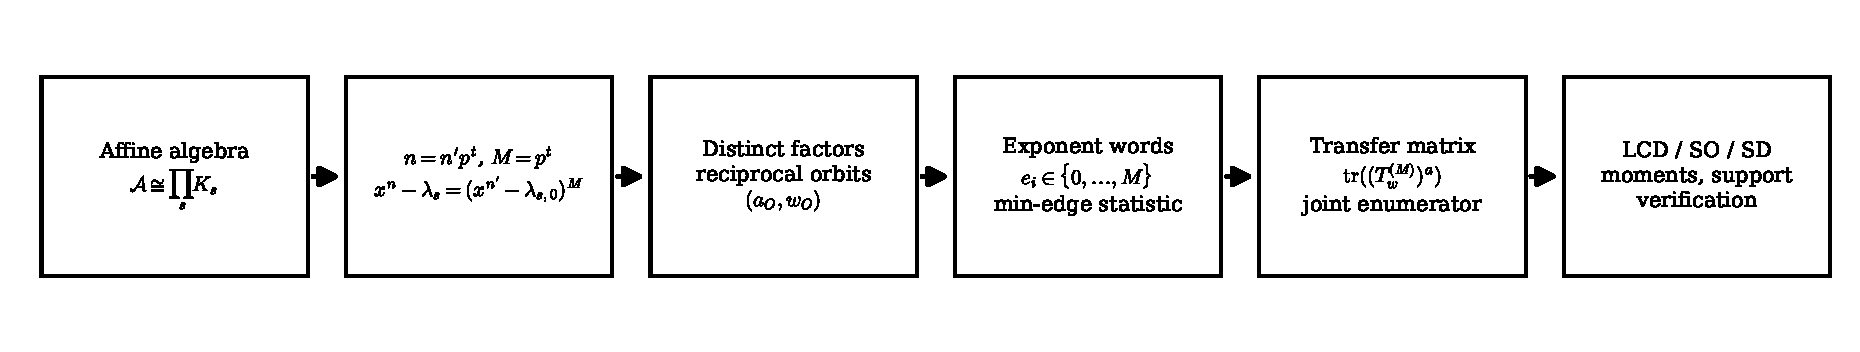
\includegraphics[width=\linewidth]{fig1_workflow.pdf}
\caption{Pipeline of the paper.}
\label{fig:workflow}
\end{figure*}

The paper is organized as follows. Section~\ref{sec:setting} introduces the
repeated-root setting, the Frobenius reduction to the square-free kernel and
the exponent-selection description of codes.
Section~\ref{sec:duality} develops $k$-Galois duality, the compatibility
criterion, reciprocal orbits and the incompatible case.
Section~\ref{sec:enumerator} proves the min-edge hull formula and the main
joint-enumerator theorem, together with its marginal and symmetry
consequences. Section~\ref{sec:consequences} derives the LCD count, exact
support, moments and conditional laws, and the self-orthogonal,
dual-containing and self-dual counts. Section~\ref{sec:examples} presents
the computation of orbit data, the exact algorithm and its complexity,
worked examples in characteristics $2$, $3$ and $5$, and independent
verification. Section~\ref{sec:conclusions} summarizes the scope of the results
and records open directions.

\section{Affine algebras and repeated-root constacyclic codes}\label{sec:setting}

The coefficient algebra in this paper is a square-free affine algebra, whereas the
code modulus is allowed to be non-square-free: we do not assume
that $\gcd(n,p)=1$, so $x^n-\lambda_s$ may have repeated irreducible factors.
The purpose of this section is to show that, over a finite field, every
repeated-root modulus is the $M$-th power of a square-free kernel, where
$M=p^{v_p(n)}$. A code is therefore determined by one exponent in
$\{0,\dots,M\}$ at each distinct irreducible factor of that kernel.

\subsection{Square-free affine algebras and their components}\label{sec:setup}

Throughout, $p$ is a prime and
\[
q=p^e,\qquad e\geq 1.
\]
For each component index $s$ we write
\[
K_s=\F_{q^{m_s}}=\F_{p^{d_s}},\qquad d_s=em_s,\qquad m_s\geq 1.
\]
The ambient algebra is
\begin{equation}\label{eq:algebra}
\A=\F_q[X_1,\ldots,X_\ell]
 \big/\langle t_1(X_1),\ldots,t_\ell(X_\ell)\rangle,
\end{equation}
where $\ell\geq1$ and every $t_i$ is monic, square-free, and of positive degree.

\begin{proposition}[Square-free component decomposition]\label{prop:decomposition}
The algebra \eqref{eq:algebra} has a fixed labeled decomposition
\begin{equation}\label{eq:decomp}
\A\cong\prod_{s=1}^{N}K_s .
\end{equation}
\end{proposition}

\begin{proof}
Each $t_i$ is separable, so factoring it into pairwise coprime monic irreducibles
and applying the Chinese remainder theorem exhibits
$\F_q[X_i]/\langle t_i\rangle$ as a finite product of finite field extensions of
$\F_q$.  The algebra \eqref{eq:algebra} is the tensor product over $\F_q$ of
these one-variable quotients; a tensor product of finite \'{e}tale algebras is
finite \'{e}tale, and a finite \'{e}tale algebra over a finite field is a finite
product of finite fields.  Fixing the tensor factors and the Chinese remainder
idempotents fixes the component labels in \eqref{eq:decomp}.
\end{proof}

We fix the decomposition \eqref{eq:decomp} once and for all and write elements of
$\A$ as tuples $(a_s)_s$.  Let $\varepsilon_s\in\A$ be the primitive idempotent
with $1$ in component $s$ and $0$ elsewhere.  Dimensions of global objects are
taken over $\F_q$; a $K_s$-dimension is converted to an $\F_q$-dimension by
multiplication by $m_s=[K_s:\F_q]$.  Thus
$\dim_{\F_q}\A=\sum_{s=1}^{N}m_s$.

It is important to keep the two uses of ``square-free'' separate: the algebra
$\A$ is square-free (reduced), whereas from \S\ref{sec:factorisation} onwards the
code modulus $x^n-\lambda_s$ is allowed, and intended, to be non-square-free.

\subsection{Constacyclic codes over \texorpdfstring{$\A$}{A}}\label{sec:codes}

Fix an arbitrary length $n\geq1$ and a twist
$\lambda=(\lambda_s)_{s=1}^{N}\in\A^\ast$, so $\lambda_s\in K_s^\ast$ for every
$s$ (throughout, $\A^\ast$ and $K_s^\ast$ denote the unit groups).  The $\lambda$-constacyclic shift on $\A^n$ is
\[
T_\lambda(c_0,c_1,\ldots,c_{n-1})
   =(\lambda c_{n-1},c_0,\ldots,c_{n-2}).
\]

\begin{definition}\label{def:constacyclic}
An \emph{$\A$-linear $\lambda$-constacyclic code} of length $n$ over $\A$ is an
$\A$-submodule $C\subseteq\A^n$ such that $T_\lambda(C)\subseteq C$.
\end{definition}

Identify $(c_0,\ldots,c_{n-1})$ with $\sum_{i=0}^{n-1}c_ix^i$.  Under this
identification $\A^n$ becomes the quotient ring
\[
R_{\A,\lambda}=\A[x]/\langle x^n-\lambda\rangle,
\]
multiplication by $x$ corresponds to $T_\lambda$, and the $\A$-linear
$\lambda$-constacyclic codes are exactly the ideals of $R_{\A,\lambda}$.
Coefficientwise, the decomposition \eqref{eq:decomp} gives
\[
R_{\A,\lambda}\cong\prod_{s=1}^{N}K_s[x]/\langle x^n-\lambda_s\rangle .
\]

\begin{lemma}\label{lem:components}
Every $\A$-linear $\lambda$-constacyclic code decomposes uniquely as a product
$C=\prod_{s=1}^{N}C_s$, where $C_s$ is an ideal of
$K_s[x]/\langle x^n-\lambda_s\rangle$.  Conversely, every such product is an
$\A$-linear $\lambda$-constacyclic code.
\end{lemma}

\begin{proof}
Multiplication by $\varepsilon_s$ projects $R_{\A,\lambda}$ onto its $s$-th
component ring.  If $C$ is an ideal, then $\varepsilon_s C$ is an ideal of the
$s$-th component; since $1=\sum_s\varepsilon_s$ is an orthogonal idempotent
decomposition, $C=\bigoplus_s\varepsilon_s C$, which is the asserted product
decomposition.  The converse is immediate from the product ring structure.
\end{proof}

\begin{remark}\label{rem:Alinear}
Definition~\ref{def:constacyclic} requires $\A$-linearity, not merely
$\F_q$-linearity plus shift-invariance.  This convention is essential for
Lemma~\ref{lem:components}: subspaces that mix the labeled components are
not counted in this paper.
\end{remark}

Nothing in Definition~\ref{def:constacyclic} or Lemma~\ref{lem:components}
requires $\gcd(n,p)=1$.  The only place where the characteristic interacts with
the length is the factorization of the component moduli, to which we now turn.

\subsection{The repeated-root factorization}\label{sec:factorisation}

Write the length as
\[
n=n'p^t,\qquad t=v_p(n)\geq0,\qquad \gcd(n',p)=1,
\]
and put
\[
M=p^t .
\]
We call $M$ the \emph{multiplicity}; the reason is Lemma~\ref{lem:factorisation}.
For each $s$, the map $a\mapsto a^M=a^{p^t}$ is a power of Frobenius, hence an
automorphism of $K_s$.  Let $\lambda_{s,0}$ be the unique element of $K_s^\ast$
such that
\begin{equation}\label{eq:lambda0}
\lambda_{s,0}^{\,M}=\lambda_s,
\qquad\text{i.e.}\qquad
\lambda_{s,0}=\Frob^{-t}(\lambda_s).
\end{equation}
Define the component modulus and its square-free kernel by
\[
P_s(x)=x^n-\lambda_s,\qquad P_{s,0}(x)=x^{n'}-\lambda_{s,0}.
\]
We deliberately write $P_s$ for the modulus, since the letter $M$ is reserved
for the multiplicity.

\begin{lemma}[Repeated-root factorization]\label{lem:factorisation}
For every component $s$,
\begin{equation}\label{eq:factorisation}
x^n-\lambda_s=\bigl(x^{n'}-\lambda_{s,0}\bigr)^M .
\end{equation}
Moreover $x^{n'}-\lambda_{s,0}$ is square-free.  Hence every distinct monic
irreducible factor of $x^n-\lambda_s$ over $K_s$ occurs with multiplicity
exactly $M$.
\end{lemma}

\begin{proof}
In characteristic $p$, the Frobenius identity
$(u-v)^{p^t}=u^{p^t}-v^{p^t}$ holds in any commutative $K_s$-algebra.  Applying
it to $u=x^{n'}$ and $v=\lambda_{s,0}$ and using \eqref{eq:lambda0} gives
\[
\bigl(x^{n'}-\lambda_{s,0}\bigr)^M
   =x^{n'p^t}-\lambda_{s,0}^{\,p^t}=x^n-\lambda_s .
\]
For square-freeness, the derivative of $P_{s,0}$ is $n'x^{n'-1}$ (equal to $1$
when $n'=1$).  A common root $\alpha$ of $P_{s,0}$ and its derivative in an
algebraic closure would satisfy $\alpha^{n'}=\lambda_{s,0}\neq0$, hence
$\alpha\neq0$, and $n'\alpha^{n'-1}=0$, contradicting $\gcd(n',p)=1$.
Thus $\gcd(P_{s,0},P_{s,0}')=1$, so $P_{s,0}$ is separable and therefore
square-free.  Raising a square-free factorization to the $M$-th power gives
every distinct irreducible factor multiplicity exactly $M$.
\end{proof}

Let
\[
\Fs=\{\text{distinct monic irreducible factors of }P_{s,0}\text{ over }K_s\}.
\]
By Lemma~\ref{lem:factorisation}, $\Fs$ is also the set of distinct monic
irreducible factors of $P_s$, and
\[
P_s(x)=\prod_{f\in\Fs}f(x)^M .
\]
The factorization theory needed here is exhausted by
Lemma~\ref{lem:factorisation}: over a finite field there are no other
multiplicity patterns for a constacyclic modulus, and no hypothesis on the
multiplicative order of $\lambda_s$ is used.

\begin{remark}\label{rem:lambda0}
The generator of a code divides $x^n-\lambda_s$, but every computation (factor
set, reciprocal action, examples) is performed with $x^{n'}-\lambda_{s,0}$.
Accordingly, every example in this paper records both $\lambda_{s,0}$ and
$\lambda_s=\lambda_{s,0}^M$.
\end{remark}

\subsection{Exponent selections}\label{sec:selections}

Fix a component $s$.  An \emph{exponent selection} is a tuple
$\mathbf{e}=(e_f)_{f\in\Fs}$ with integers
\[
0\leq e_f\leq M\qquad(f\in\Fs).
\]
(The bold $\mathbf{e}$ denotes the selection; its coordinates are the $e_f$.
The plain letter $e$ continues to denote the exponent in $q=p^e$.)  Set
\[
g_{\mathbf{e}}=\prod_{f\in\Fs}f^{e_f},
\qquad
h_{\mathbf{e}}=\frac{P_s}{g_{\mathbf{e}}}
   =\prod_{f\in\Fs}f^{M-e_f},
\]
and let $C_s(\mathbf{e})=\langle g_{\mathbf{e}}\rangle\subseteq
K_s[x]/\langle P_s\rangle$.

\begin{lemma}\label{lem:component-selection}
The $\lambda_s$-constacyclic codes in $K_s[x]/\langle P_s\rangle$ are exactly
the ideals $C_s(\mathbf{e})$, and distinct exponent selections give distinct
codes.  Moreover
\begin{equation}\label{eq:component-dim}
\dim_{K_s}C_s(\mathbf{e})
   =n-\sum_{f\in\Fs}e_f\deg f
   =\sum_{f\in\Fs}(M-e_f)\deg f .
\end{equation}
\end{lemma}

\begin{proof}
Since $K_s[x]$ is a principal ideal domain, the ideals of the quotient
$K_s[x]/\langle P_s\rangle$ are the principal ideals generated by the monic
divisors of $P_s$, each monic divisor determining a distinct ideal.  By
Lemma~\ref{lem:factorisation}, a monic divisor of
$P_s=\prod_{f\in\Fs}f^M$ is precisely a choice of exponents
$e_f\in\{0,\ldots,M\}$, and unique factorization makes the correspondence
bijective.  The ideal generated by a polynomial of degree $d$ in a quotient by a
degree-$n$ modulus has $K_s$-dimension $n-d$; with
$d=\deg g_{\mathbf{e}}=\sum_f e_f\deg f$ and $n=M\sum_f\deg f$ this gives both
forms in \eqref{eq:component-dim}.
\end{proof}

Globally, write a selection as
$\mathbf{e}=(\mathbf{e}^{(s)})_{s=1}^{N}$ and put
$C(\mathbf{e})=\prod_{s=1}^{N}C_s(\mathbf{e}^{(s)})$.  Set
\[
N_F=\sum_{s=1}^{N}|\Fs|,
\qquad
W=n\sum_{s=1}^{N}m_s=\dim_{\F_q}\A^n .
\]
For a global code $C$ we write $\kappa(C)=\dim_{\F_q}C$.

\begin{proposition}\label{prop:global-selection}
The map $\mathbf{e}\mapsto C(\mathbf{e})$ is a bijection from
$\prod_{s=1}^{N}\{0,\ldots,M\}^{\Fs}$ to the set of $\A$-linear
$\lambda$-constacyclic codes of length $n$ over $\A$.  In particular the number
of labeled codes is $(M+1)^{N_F}$, and
\begin{equation}\label{eq:kappa}
\kappa(C(\mathbf{e}))
   =\sum_{s=1}^{N}\sum_{f\in\Fs}m_s(\deg f)\,(M-e_f).
\end{equation}
\end{proposition}

\begin{proof}
By Lemma~\ref{lem:components} a global code is a product of component ideals,
and by Lemma~\ref{lem:component-selection} each component ideal is determined
by a unique exponent selection.  This proves the bijection and the count
$(M+1)^{N_F}$.  Formula \eqref{eq:kappa} is \eqref{eq:component-dim} summed
over components, with each $K_s$-dimension multiplied by $m_s$.
\end{proof}

The extreme selections are $\mathbf{e}=(M,\ldots,M)$, giving the zero code, and
$\mathbf{e}=(0,\ldots,0)$, giving the whole ambient space, of $\F_q$-dimension
$W$.  Counting throughout is \emph{labeled}: distinct exponent selections are
counted separately, with no quotient by any equivalence relation.  In
probabilistic statements, ``uniform'' always refers to the uniform measure on
the $(M+1)^{N_F}$ exponent selections.

Thus each distinct irreducible factor contributes one exponent coordinate,
with the $M+1$ possible values $0,1,\ldots,M$.

\section{\texorpdfstring{$k$}{k}-Galois duality}\label{sec:duality}

This section develops $k$-Galois duality directly for the exponent
selections of Proposition~\ref{prop:global-selection}.  The Euclidean dual
generator is verified for arbitrary length in
Lemma~\ref{lem:euclidean-dual}.  The outcome is an explicit compatibility
condition for each component; under compatibility, the reciprocal permutes
the distinct kernel factors, and multiplicities enter the dual generator
through the identity $(f^m)^{\#}=(f^{\#})^m$.

\subsection{Pairings, duals and hulls}\label{sec:pairing}

Fix an integer $k$ with $0\leq k<e$.  On $K_s$ put
\[
\sigma_{s,k}(a)=a^{p^k},\qquad
\rho_{s,k}(a)=a^{p^{d_s-k}}=\sigma_{s,k}^{-1}(a).
\]
The \emph{component $k$-Galois pairing} on $K_s^n$ is
\begin{equation}\label{eq:pairing}
\langle x,y\rangle_{s,k}
   =\sum_{i=0}^{n-1}x_i\,\sigma_{s,k}(y_i)
   =\sum_{i=0}^{n-1}x_i y_i^{p^k}.
\end{equation}
It is $K_s$-linear in the first argument and $\sigma_{s,k}$-semilinear in the
second; note that it is \emph{code-first} in the sense of
Remark~\ref{rem:candidate}.  For a $K_s$-linear code $C\subseteq K_s^n$ define
\[
\Dk(C)=\bigl\{y\in K_s^n:\langle c,y\rangle_{s,k}=0
 \text{ for every }c\in C\bigr\},
\qquad
\Hull_k(C)=C\cap\Dk(C),
\]
the \emph{$k$-Galois dual} and \emph{$k$-Galois hull}.  The annihilator
$\Dk(C)$ is a $K_s$-subspace: if $y\in\Dk(C)$ and $a\in K_s$, then
$\langle c,ay\rangle_{s,k}=\sigma_{s,k}(a)\langle c,y\rangle_{s,k}=0$.

Componentwise Frobenius gives mutually inverse ring automorphisms
$\sigma_{\A,k},\rho_{\A,k}$ of $\A$, and the \emph{global $k$-Galois pairing} on
$\A^n$ is the $\A$-valued pairing
\[
\langle x,y\rangle_{\A,k}
   =\sum_{i=0}^{n-1}x_i\,\sigma_{\A,k}(y_i)
   =\Bigl(\sum_{i=0}^{n-1}x_{s,i}y_{s,i}^{p^k}\Bigr)_{s=1}^{N}.
\]
The global dual and hull $D_{\A,k}(C)$ and $\Hull_{\A,k}(C)$ are defined by the
same annihilator formulas with $\langle\cdot,\cdot\rangle_{\A,k}$.  For a
global code $C$ we write
\[
\eta_k(C)=\dim_{\F_q}\Hull_{\A,k}(C).
\]

\begin{lemma}\label{lem:global-duality}
If $C=\prod_{s=1}^{N}C_s$ is a product code, then
\[
D_{\A,k}(C)=\prod_{s=1}^{N}\Dk(C_s),
\qquad
\Hull_{\A,k}(C)=\prod_{s=1}^{N}\Hull_k(C_s),
\]
and consequently
$\eta_k(C)=\sum_{s=1}^{N}m_s\dim_{K_s}\Hull_k(C_s)$.
\end{lemma}

\begin{proof}
An element of $\A$ is zero if and only if every component is zero, so
$\langle c,y\rangle_{\A,k}=0$ if and only if
$\langle c_s,y_s\rangle_{s,k}=0$ for all $s$.  Taking for $c$ a codeword
supported in a single component shows $y_s\in\Dk(C_s)$ for every $s$; the
converse inclusion is immediate.  Intersections of product sets are products of
intersections, giving the hull statement, and the dimension formula is the
usual conversion by $m_s$.
\end{proof}

Lemma~\ref{lem:global-duality} is a product argument and is indifferent to
whether $p$ divides $n$; the same is true of the next statement, which reduces
$k$-Galois duality to Euclidean duality.

\begin{proposition}\label{prop:dual-translation}
For every $K_s$-linear code $C\subseteq K_s^n$,
\[
\Dk(C)=\rho_{s,k}\bigl(C^{\perpE}\bigr),
\]
where $C^{\perpE}$ is the ordinary Euclidean dual and $\rho_{s,k}$ acts
coordinatewise.
\end{proposition}

\begin{proof}
The defining condition for $y\in\Dk(C)$ is
$\sum_i c_i\sigma_{s,k}(y_i)=0$ for all $c\in C$.  Putting
$z=\sigma_{s,k}(y)$ coordinatewise, this says $z\in C^{\perpE}$, and applying
the inverse map $\rho_{s,k}$ coordinatewise gives $y=\rho_{s,k}(z)$.
\end{proof}

\begin{remark}\label{rem:euclidean-hermitian}
For $k=0$ the pairing \eqref{eq:pairing} is Euclidean on every component.  On
$K_s=\F_{p^{d_s}}$ it is Hermitian if and only if $d_s$ is even and
$k\equiv d_s/2\pmod{d_s}$; in particular, when $e$ is even the base-field
choice $k=e/2$ is Hermitian only on components with $m_s=1$, not in general.
We therefore avoid the unqualified phrase ``the Hermitian case''.
\end{remark}

We use the standard terminology, componentwise or globally according to
context: a code is \emph{$k$-Galois LCD} (linear with complementary dual) if
$\Hull_k(C)=\{0\}$, \emph{self-orthogonal} if $C\subseteq\Dk(C)$,
\emph{dual-containing} if $\Dk(C)\subseteq C$, and \emph{self-dual} if
$C=\Dk(C)$ as subspaces (no involutivity of $\Dk$ is assumed).

\subsection{The inverse-Frobenius reciprocal}\label{sec:reciprocal}

Let $f(x)=\sum_{i=0}^{r}f_ix^i\in K_s[x]$ be monic with $f_0\neq0$.  The
\emph{normalized inverse-Frobenius reciprocal} of $f$ is
\begin{equation}\label{eq:reciprocal}
f^{\#_{s,k}}(x)
   =\rho_{s,k}(f_0)^{-1}\sum_{i=0}^{r}\rho_{s,k}(f_i)x^{r-i}.
\end{equation}
For $k=0$ this is the ordinary normalized reciprocal, which we also denote by
$f^\ast$ when the field is arbitrary.

\begin{lemma}\label{lem:reciprocal}
The map $f\mapsto f^{\#_{s,k}}$ on monic polynomials with nonzero constant term
is monic and degree-preserving, is multiplicative, hence satisfies
$(f^m)^{\#_{s,k}}=(f^{\#_{s,k}})^m$ for every $m\geq0$, preserves
irreducibility, and is inverted by the corresponding normalized reciprocal with
$\sigma_{s,k}$ in place of $\rho_{s,k}$.
\end{lemma}

\begin{proof}
Reversal puts $\rho_{s,k}(f_0)\neq0$ in degree $r$, so the normalization in
\eqref{eq:reciprocal} makes $f^{\#_{s,k}}$ monic of degree $r$; its constant
term is $\rho_{s,k}(f_r)/\rho_{s,k}(f_0)=\rho_{s,k}(f_0)^{-1}\neq0$.  If
$\widetilde{f}=\sum_i\rho_{s,k}(f_i)x^{r-i}$ denotes the unnormalized reversal,
then $\widetilde{fg}=\widetilde{f}\,\widetilde{g}$ for monic $f,g$ with nonzero
constant terms, because coefficient reversal and the ring homomorphism
$\rho_{s,k}$ are both multiplicative; the normalizing constants multiply as
$\rho_{s,k}(f_0g_0)^{-1}=\rho_{s,k}(f_0)^{-1}\rho_{s,k}(g_0)^{-1}$, proving
multiplicativity and in particular the power identity.  Applying instead the
normalized reciprocal built from $\sigma_{s,k}$ reverses the coefficients a
second time and applies $\sigma_{s,k}\rho_{s,k}=\mathrm{id}$; since the constant
term of $f^{\#_{s,k}}$ is $\rho_{s,k}(f_0)^{-1}$, the second normalization
restores $f$, so the map is bijective with the stated inverse.  Finally, a
nontrivial monic factorization $f=gh$ maps under the multiplicative bijection
to a nontrivial factorization of $f^{\#_{s,k}}$, and conversely via the inverse;
hence irreducibility is preserved.
\end{proof}

\begin{lemma}\label{lem:root-action}
Let $f$ be as above and let $\alpha$ be a root of $f$ in an extension field.
Then $\alpha^{-p^{d_s-k}}$ is a root of $f^{\#_{s,k}}$.
\end{lemma}

\begin{proof}
Since $f_0\neq0$ we have $\alpha\neq0$.  Extend $\rho=\rho_{s,k}$ to the
extension field by $\rho(a)=a^{p^{d_s-k}}$.  From \eqref{eq:reciprocal},
\[
f^{\#_{s,k}}(x)=\rho(f_0)^{-1}x^r\sum_{i=0}^{r}\rho(f_i)x^{-i}.
\]
Put $\beta=\rho(\alpha^{-1})=\alpha^{-p^{d_s-k}}$, so
$\beta^{-1}=\rho(\alpha)$.  Then
\[
\sum_{i=0}^{r}\rho(f_i)\beta^{-i}
   =\sum_{i=0}^{r}\rho(f_i)\rho(\alpha)^i
   =\rho\Bigl(\sum_{i=0}^{r}f_i\alpha^i\Bigr)=\rho(f(\alpha))=0,
\]
hence $f^{\#_{s,k}}(\beta)=0$.
\end{proof}

\subsection{Euclidean and \texorpdfstring{$k$}{k}-Galois dual
generators}\label{sec:dual-generators}

We first verify the Euclidean dual generator for arbitrary length $n$.

\begin{lemma}\label{lem:euclidean-dual}
Let $K$ be a finite field, $a\in K^\ast$ and $n\geq1$ arbitrary.  Let
$G\mid x^n-a$ be monic, put $H=(x^n-a)/G$, and let $H^\ast$ be the ordinary
normalized reciprocal of $H$.  Then the Euclidean dual of the ideal
$\langle G\rangle$ in $K[x]/\langle x^n-a\rangle$ is the
$a^{-1}$-constacyclic ideal generated by $H^\ast$.
\end{lemma}

\begin{proof}
Write $r=\deg G$ and $d_H=\deg H$, so $r+d_H=n$; note $H(0)\neq0$ since
$G(0)H(0)=-a\neq0$, so $H^\ast$ is defined (and equals $1$ if $d_H=0$).  The
non-wrapped shifts $x^iG$, $0\leq i<d_H$, form a basis of $\langle G\rangle$,
and we compare them with the non-wrapped shifts $x^jH^\ast$, $0\leq j<r$.  The
Euclidean pairing of $x^iG$ and $x^jH^\ast$ is, up to the nonzero scalar
$H(0)^{-1}$, the coefficient of $x^{d_H-i+j}$ in $GH$: indeed, reversal sends
the coefficient $H_u$ of $H$ to degree $d_H-u$ in $H^\ast$, so aligned terms in
the pairing have $u+v=d_H-i+j$ where $v$ indexes coefficients of $G$.  Since
$1\leq d_H-i+j\leq n-1$ and $GH=x^n-a$ has no terms in these degrees, the
pairing is zero.  Thus the two shift spaces are mutually orthogonal.

By multiplicativity of the ordinary reciprocal and
$(x^n-a)^\ast=x^n-a^{-1}$ we have $H^\ast\mid x^n-a^{-1}$, so the shifts
$x^jH^\ast$ span the $a^{-1}$-constacyclic ideal generated by $H^\ast$, of
dimension $r$.  This equals the codimension of $\langle G\rangle$; an
orthogonal space of the codimension is the dual.  The boundary cases
$r=0$ and $d_H=0$ are included: they give the zero ideal generated by
$H^\ast=x^n-a^{-1}$ in its quotient, and the whole space generated by
$H^\ast=1$, respectively.

No step uses that $x^n-a$ is square-free, or that $\gcd(n,\operatorname{char}K)=1$:
the argument sees only the identity $GH=x^n-a$ and a dimension count, and any
multiplicities are carried along inside $H$.
\end{proof}

Applying Proposition~\ref{prop:dual-translation} to
Lemma~\ref{lem:euclidean-dual} gives the $k$-Galois dual generator.  Note that
applying $\rho_{s,k}$ to the coefficients of the ordinary reciprocal $h^\ast$
gives exactly $h^{\#_{s,k}}$ as defined in \eqref{eq:reciprocal}.

\begin{theorem}\label{thm:dual-generator}
Let $C_s(\mathbf{e})=\langle g_{\mathbf{e}}\rangle$ be a component code and
$h_{\mathbf{e}}=P_s/g_{\mathbf{e}}=\prod_{f\in\Fs}f^{M-e_f}$.  Then
$\Dk(C_s(\mathbf{e}))$ is the constacyclic ideal generated by
$h_{\mathbf{e}}^{\#_{s,k}}$, with dual twist
\[
\mu_s=\lambda_s^{-p^{d_s-k}}.
\]
\end{theorem}

\begin{proof}
By Proposition~\ref{prop:dual-translation},
$\Dk(C_s(\mathbf{e}))=\rho_{s,k}(C_s(\mathbf{e})^{\perpE})$ with $\rho_{s,k}$
acting coordinatewise, i.e.\ coefficientwise on polynomial representatives.
By Lemma~\ref{lem:euclidean-dual} the Euclidean dual is the
$\lambda_s^{-1}$-constacyclic ideal generated by $h_{\mathbf{e}}^\ast$.
Coefficientwise application of $\rho_{s,k}$ sends generator
$h_{\mathbf{e}}^\ast$ to $h_{\mathbf{e}}^{\#_{s,k}}$ and twist $\lambda_s^{-1}$
to $\rho_{s,k}(\lambda_s^{-1})=\lambda_s^{-p^{d_s-k}}=\mu_s$.
\end{proof}

\subsection{Compatibility and incompatible twists}\label{sec:compatibility}

The dual twist in Theorem~\ref{thm:dual-generator} need not equal $\lambda_s$.
We now determine exactly when it does.  Since all factor computations take place
in the base modulus $P_{s,0}$, we first compute its reciprocal: directly from
\eqref{eq:reciprocal},
\begin{equation}\label{eq:base-reciprocal}
P_{s,0}^{\#_{s,k}}
   =x^{n'}-\lambda_{s,0}^{-p^{d_s-k}}.
\end{equation}
Call the component $s$ \emph{compatible} (for the given $k$) if
$f\mapsto f^{\#_{s,k}}$ permutes $\Fs$, and call $\lambda$ \emph{compatible} if
every component is.

\begin{proposition}\label{prop:compatibility}
For each component $s$ the following are equivalent:
\begin{enumerate}
\item[\textup{(i)}] $s$ is compatible;
\item[\textup{(ii)}] $\lambda_{s,0}^{\,1+p^{d_s-k}}=1$;
\item[\textup{(iii)}] $\lambda_s^{\,1+p^{d_s-k}}=1$.
\end{enumerate}
In particular the compatibility condition is the same for $\lambda_{s,0}$ and
for $\lambda_s=\lambda_{s,0}^M$.
\end{proposition}

\begin{proof}
Let $f\in\Fs$.  By Lemma~\ref{lem:reciprocal}, $f^{\#_{s,k}}$ is monic
irreducible, and since $f\mid P_{s,0}$, multiplicativity gives
$f^{\#_{s,k}}\mid P_{s,0}^{\#_{s,k}}$, which by \eqref{eq:base-reciprocal} is
$x^{n'}-\lambda_{s,0}^{-p^{d_s-k}}$.  If (ii) holds, then
$\lambda_{s,0}^{-p^{d_s-k}}=\lambda_{s,0}$, so
$P_{s,0}^{\#_{s,k}}=P_{s,0}$ and $f^{\#_{s,k}}\in\Fs$; the inverse map of
Lemma~\ref{lem:reciprocal} then makes $f\mapsto f^{\#_{s,k}}$ a permutation of
$\Fs$, giving (i).  Conversely, if (i) holds, applying $\#_{s,k}$ to the
square-free product $P_{s,0}=\prod_{f\in\Fs}f$ gives
$P_{s,0}^{\#_{s,k}}=\prod_{f\in\Fs}f^{\#_{s,k}}=P_{s,0}$; comparing with
\eqref{eq:base-reciprocal} yields
$\lambda_{s,0}^{-p^{d_s-k}}=\lambda_{s,0}$, which is (ii).

For (ii)$\Leftrightarrow$(iii), put $c=1+p^{d_s-k}$.  Then
$\lambda_s^c=(\lambda_{s,0}^M)^c=(\lambda_{s,0}^c)^M$.  The map
$y\mapsto y^M=y^{p^t}$ on $K_s^\ast$ is a Frobenius power, hence injective with
$1^M=1$; therefore $(\lambda_{s,0}^c)^M=1$ if and only if
$\lambda_{s,0}^c=1$.
\end{proof}

Under compatibility we define
\[
\tau_{s,k}:\Fs\longrightarrow\Fs,\qquad \tau_{s,k}(f)=f^{\#_{s,k}},
\]
a degree-preserving permutation by Lemma~\ref{lem:reciprocal}; it need not be
an involution.  Condition (iii) is exactly $\mu_s=\lambda_s$, so by
Theorem~\ref{thm:dual-generator} the $k$-Galois dual is again
$\lambda_s$-constacyclic, and its generator can be read off factor by factor.

\begin{proposition}\label{prop:dual-exponents}
If $s$ is compatible, then for every exponent selection $\mathbf{e}$,
\begin{equation}\label{eq:dual-exponents}
h_{\mathbf{e}}^{\#_{s,k}}
   =\prod_{f\in\Fs} f^{\,M-e_{\tau_{s,k}^{-1}(f)}}.
\end{equation}
In words: the exponent of $f$ in the dual generator is $M$ minus the exponent
of its $\tau_{s,k}$-predecessor in $g_{\mathbf{e}}$.
\end{proposition}

\begin{proof}
By multiplicativity and the power identity in Lemma~\ref{lem:reciprocal},
\[
h_{\mathbf{e}}^{\#_{s,k}}
 =\prod_{f\in\Fs}\bigl(f^{M-e_f}\bigr)^{\#_{s,k}}
 =\prod_{f\in\Fs}\tau_{s,k}(f)^{\,M-e_f}.
\]
Re-indexing by $g=\tau_{s,k}(f)$ gives \eqref{eq:dual-exponents}.
\end{proof}

\begin{remark}\label{rem:special-twists}
The twists $\lambda_s=1$ (cyclic) and $\lambda_s=-1$ (negacyclic) are always
compatible: for odd $p$, $(-1)^{1+p^{d_s-k}}=1$ because $p^{d_s-k}$ is odd, and
for $p=2$ one has $-1=1$.
\end{remark}

It remains to dispose of the incompatible components.  They turn out to be
enumeration-theoretically trivial.

\begin{proposition}\label{prop:incompatible}
If the component $s$ is incompatible, then
$\Hull_k(C_s(\mathbf{e}))=\{0\}$ for every exponent selection $\mathbf{e}$; in
particular every such component code is $k$-Galois LCD.
\end{proposition}

\begin{proof}
By Proposition~\ref{prop:compatibility} and Theorem~\ref{thm:dual-generator},
incompatibility means $\mu_s=\lambda_s^{-p^{d_s-k}}\neq\lambda_s$, the generator
$g_{\mathbf{e}}$ divides $x^n-\lambda_s$, and the dual generator
$h_{\mathbf{e}}^{\#_{s,k}}$ divides $x^n-\mu_s$.  The two moduli differ by the
nonzero constant $\mu_s-\lambda_s$, hence are coprime; therefore
$\gcd(g_{\mathbf{e}},h_{\mathbf{e}}^{\#_{s,k}})=1$.  Moreover
$\deg g_{\mathbf{e}}+\deg h_{\mathbf{e}}^{\#_{s,k}}
 =\deg g_{\mathbf{e}}+\deg h_{\mathbf{e}}=n$.
A hull codeword has a unique representative polynomial of degree $<n$; that
representative is divisible in $K_s[x]$ both by $g_{\mathbf{e}}$ (since it lies
in $C_s(\mathbf{e})$) and by $h_{\mathbf{e}}^{\#_{s,k}}$ (since it lies in the
dual, whose words are the multiples of its generator of degree $<n$).  Being
divisible by two coprime polynomials whose degrees sum to $n$, it is divisible
by a polynomial of degree $n$, hence is zero.
\end{proof}

\begin{corollary}\label{cor:incompatible}
Let $s$ be incompatible.  Then the component contributes $0$ to every global
hull dimension.  The only self-orthogonal component code is $\{0\}$, the only
dual-containing component code is $K_s^n$, and there is no self-dual component
code.
\end{corollary}

\begin{proof}
The first statement is Proposition~\ref{prop:incompatible} combined with
Lemma~\ref{lem:global-duality}.  If $C_s(\mathbf{e})$ is self-orthogonal then
$C_s(\mathbf{e})=\Hull_k(C_s(\mathbf{e}))=\{0\}$.  If it is dual-containing then
$\Dk(C_s(\mathbf{e}))=\Hull_k(C_s(\mathbf{e}))=\{0\}$, and by
Proposition~\ref{prop:dual-translation}
$\dim_{K_s}\Dk(C_s(\mathbf{e}))=n-\dim_{K_s}C_s(\mathbf{e})$, forcing
$C_s(\mathbf{e})=K_s^n$.  Self-duality would give
$C_s(\mathbf{e})=\Hull_k(C_s(\mathbf{e}))=\{0\}$ and at the same time
$\Dk(C_s(\mathbf{e}))=\{0\}$, impossible for $n\geq1$.
\end{proof}

\begin{example}\label{ex:incompatible}
Let $K_s=\F_5$, $n'=2$, $M=5$, so $n=10$, and take $k=0$ and
$\lambda_{s,0}=\lambda_s=2$.  Then $x^2-2$ is irreducible over $\F_5$ (the
nonzero squares are $1,4$), so $\Fs=\{x^2-2\}$, and
$\lambda_s^{1+5}=2^6=4\neq1$ in $\F_5$: the component is incompatible.  The six
codes $\langle(x^2-2)^e\rangle$, $e=0,\ldots,5$, therefore have
$(\kappa,\eta_0)=(10-2e,0)$ by Proposition~\ref{prop:incompatible}.
\end{example}

\begin{remark}\label{rem:candidate}
Part of the literature uses the \emph{candidate-first} dual
$D_{\mathrm{cand}}(C)=\{y:\sum_i y_i\sigma_{s,k}(c_i)=0\text{ for all }c\in C\}$.
Substituting $y=\sigma_{s,k}(z)$ gives
$\sum_i y_i\sigma_{s,k}(c_i)=\sigma_{s,k}(\sum_i z_ic_i)$, hence
$D_{\mathrm{cand}}(C)=\sigma_{s,k}(C^{\perpE})$, and therefore
$D_{\mathrm{cand}}(C)=\sigma_{s,k}^2(\Dk(C))$ by
Proposition~\ref{prop:dual-translation}.  The two duals are different subspaces
in general; generator and factor-support statements in this paper refer to the
code-first dual \eqref{eq:pairing}.  Hull \emph{dimensions}, however, agree:
if $B$ is a row basis of $C$ and $G=B\,\sigma_{s,k}(B)^{\mathsf T}$, then for
$y=vB$ the code-first hull condition is $G\,\sigma_{s,k}(v)^{\mathsf T}=0$ and
the candidate-first condition is $vG=0$; right and left nullspaces have the
same dimension $\dim C-\rank G$.  Thus every hull-dimension statement below is
convention-independent, and the Gram-matrix rank identity just displayed is
what our independent computational verification in
Section~\ref{sec:examples} implements.
\end{remark}

We have now covered every twist $\lambda$: incompatible components contribute
no hull dimension at all, and compatible components are governed by the
permutation $\tau_{s,k}$ and the dual exponents
\eqref{eq:dual-exponents}.  The next section turns this into an explicit
formula for $\eta_k(C(\mathbf{e}))$ and then into the joint enumerator.

\section{Hull statistic and the joint enumerator}\label{sec:enumerator}

We now convert the dual exponents of Section~\ref{sec:duality} into a formula
for the hull dimension and then into the joint enumerator.  Compatible
components are organized by the cycles of $\tau_{s,k}$; incompatible components
require no orbit structure, because their hull contribution is identically zero
(Proposition~\ref{prop:incompatible}).

\subsection{Reciprocal orbits and exponent words}\label{sec:orbits}

Let $s$ be a compatible component.  Denote by $\Os$ the set of cycles
(orbits) of the permutation $\tau_{s,k}$ on the \emph{distinct} factor set
$\Fs$; multiplicities do not create new factors.  For $O\in\Os$ write
\[
a_O=|O|,\qquad d_O=\text{common degree of the factors in }O,\qquad
w_O=m_sd_O .
\]
The degree is constant on $O$ by Lemma~\ref{lem:reciprocal}.  Enumerate
\[
O=(f_{O,1},\ldots,f_{O,a_O})
\qquad\text{so that}\qquad
\tau_{s,k}(f_{O,i})=f_{O,i+1},
\]
with indices modulo $a_O$.  The starting point of this enumeration is arbitrary;
its cyclic direction is the one prescribed by $\tau_{s,k}$.

The restriction of an exponent selection to $O$ is the \emph{exponent word}
\[
(e_{O,1},\ldots,e_{O,a_O})\in\{0,\ldots,M\}^{a_O},
\qquad e_{O,i}=e_{f_{O,i}} .
\]
By Proposition~\ref{prop:global-selection}, a global selection is an
independent choice of one exponent word on every compatible orbit, together
with one exponent at every distinct factor of every incompatible component.
This independence is the engine of the factorization in
Theorem~\ref{thm:main}.

For an incompatible component and $f\in\Fs$ we use the individual weight
$w_f=m_s\deg f$; on a compatible orbit, $w_f=w_O$ for every $f\in O$.

\subsection{The hull generator and the \texorpdfstring{$\min$}{min}-edge
formula}\label{sec:min-edge}

\begin{lemma}\label{lem:hull-generator}
Let $s$ be compatible and let $\mathbf{e}$ be an exponent selection.  Then
$\Hull_k(C_s(\mathbf{e}))$ is the ideal generated by
$\lcm(g_{\mathbf{e}},h_{\mathbf{e}}^{\#_{s,k}})$.  On an orbit
$O=(f_{O,1},\ldots,f_{O,a_O})$ the exponents are:
{\small
\[
\begin{array}{c|c}
\text{polynomial} & \text{exponent at }f_{O,i}\\ \hline
 g_{\mathbf{e}} & e_{O,i}\\
 h_{\mathbf{e}} & M-e_{O,i}\\
 h_{\mathbf{e}}^{\#_{s,k}} & M-e_{O,i-1}\\
 \lcm(g_{\mathbf{e}},h_{\mathbf{e}}^{\#_{s,k}}) &
   \max\{e_{O,i},\,M-e_{O,i-1}\}
\end{array}
\]
}
with indices modulo $a_O$.
\end{lemma}

\begin{proof}
Under compatibility, Theorem~\ref{thm:dual-generator} says that both
$C_s(\mathbf{e})$ and $\Dk(C_s(\mathbf{e}))$ are ideals in the same quotient
$K_s[x]/\langle P_s\rangle$, generated by the monic divisors
$g_{\mathbf{e}}$ and $h_{\mathbf{e}}^{\#_{s,k}}$ of $P_s$.  A polynomial
representative of degree $<n$ lies in both ideals if and only if it is
divisible in $K_s[x]$ by both generators, equivalently by their least common
multiple.  That least common multiple again divides $P_s$, since the exponent
of each distinct factor is a maximum of two numbers in $\{0,\ldots,M\}$.  The
table combines the definitions of $g_{\mathbf{e}}$ and $h_{\mathbf{e}}$ with
Proposition~\ref{prop:dual-exponents}, using
$\tau_{s,k}^{-1}(f_{O,i})=f_{O,i-1}$.
\end{proof}

\begin{proposition}\label{prop:min-edge}
For every exponent selection $\mathbf{e}$,
\begin{equation}\label{eq:eta-min-edge}
\eta_k(C(\mathbf{e}))
 =\sum_{s\ \mathrm{compatible}}\ \sum_{O\in\Os}
   w_O\sum_{i=1}^{a_O}\min\{e_{O,i},\,M-e_{O,i+1}\},
\end{equation}
whereas
\begin{equation}\label{eq:kappa-orbits}
\kappa(C(\mathbf{e}))
 =\sum_{s\ \mathrm{compatible}}\sum_{O\in\Os}
   w_O\sum_{i=1}^{a_O}(M-e_{O,i})
  +\sum_{s\ \mathrm{incompatible}}\sum_{f\in\Fs}w_f(M-e_f).
\end{equation}
In particular, if every component is compatible, the second sum in
\eqref{eq:kappa-orbits} is absent.
\end{proposition}

\begin{proof}
Let $s$ be compatible.  By Lemma~\ref{lem:hull-generator} and the dimension
formula for a principal ideal, the contribution of the factor $f_{O,i}$ to
$\dim_{K_s}\Hull_k(C_s(\mathbf{e}))$ is
\[
d_O\Bigl(M-\max\{e_{O,i},M-e_{O,i-1}\}\Bigr)
   =d_O\min\{e_{O,i-1},M-e_{O,i}\}.
\]
Re-indexing $i-1\mapsto i$ gives $d_O\min\{e_{O,i},M-e_{O,i+1}\}$.
Multiplying by $m_s$, summing over $i$ and over all orbits of all compatible
components, and using Proposition~\ref{prop:incompatible} for the remaining
components gives \eqref{eq:eta-min-edge} (via
Lemma~\ref{lem:global-duality}).  Formula \eqref{eq:kappa-orbits} is
\eqref{eq:kappa} regrouped by orbits on compatible components.
\end{proof}

\begin{remark}\label{rem:debnath-agreement}
For a single compatible orbit, \eqref{eq:eta-min-edge} agrees with the
one-code hull-dimension formula of Debnath et al.\
\cite{debnathAffine2026} on the range where both apply. Their expression is
in the equivalent ``max'' form
$aM-\sum_i\max\{e_i,M-e_{i-1}\}$, and the identity
$M-\max\{u,v\}=\min\{M-u,M-v\}$ converts it, term by term, into
\eqref{eq:eta-min-edge} (the hull dimension is unaffected by the
candidate-first/code-first choice of dual convention; see
Remark~\ref{rem:candidate}). No coprimality condition
$\gcd(\operatorname{ord}\lambda_s,n')=1$ is needed here: only the component
compatibility condition $\lambda_{s,0}^{1+p^{d_s-k}}=1$ matters, and
components failing it have trivial hull by
Proposition~\ref{prop:incompatible}.
\end{remark}

Thus, on one compatible orbit, $\kappa$ is a sum over the \emph{vertices} of a
directed cycle and $\eta_k$ is a sum over its \emph{directed edges}
$i\to i+1$, both scaled by $w_O$.

\subsection{Transfer matrix and the main theorem}\label{sec:transfer}

\begin{definition}\label{def:enumerator}
The \emph{joint code-dimension and $k$-Galois-hull enumerator} is
\[
\Epoly^{(M)}(U,Z)
   :=\sum_{\mathbf{e}}U^{\kappa(C(\mathbf{e}))}
                      Z^{\eta_k(C(\mathbf{e}))}
   \in\mathbb{Z}[U,Z],
\]
the sum running over all $(M+1)^{N_F}$ exponent selections.  We write
$N_{\kappa,\eta}=[U^\kappa Z^\eta]\Epoly^{(M)}(U,Z)$.
\end{definition}

By Proposition~\ref{prop:global-selection}, $N_{\kappa,\eta}$ is the number of
labeled $\A$-linear $\lambda$-constacyclic codes $C$ with
$\dim_{\F_q}C=\kappa$ and $\dim_{\F_q}\Hull_k(C)=\eta$.

Fix a compatible orbit of length $a$ and weight $w$.  Its one-orbit polynomial
is
\begin{equation}\label{eq:one-orbit-poly}
\Epoly_{a,w}^{(M)}(U,Z)
 :=\sum_{(e_1,\ldots,e_a)\in\{0,\ldots,M\}^a}
   U^{w\sum_{i=1}^{a}(M-e_i)}
   Z^{w\sum_{i=1}^{a}\min\{e_i,M-e_{i+1}\}},
\end{equation}
indices modulo $a$.  Define the $(M+1)\times(M+1)$ transfer matrix, with rows
and columns indexed by states $0,\ldots,M$, by
\begin{equation}\label{eq:transfer}
\boxed{\;
\bigl(T^{(M)}_w(U,Z)\bigr)_{\alpha,\beta}
   =U^{w(M-\beta)}Z^{w\min\{\alpha,M-\beta\}},
\qquad 0\leq\alpha,\beta\leq M.\;}
\end{equation}
The entry records the destination vertex $\beta$ in the $U$-exponent and the
directed edge $\alpha\to\beta$ in the $Z$-exponent.  For example,
\[
T^{(2)}_w(U,Z)=
\begin{pmatrix}
U^{2w} & U^w & 1\\
U^{2w}Z^w & U^wZ^w & 1\\
U^{2w}Z^{2w} & U^wZ^w & 1
\end{pmatrix}.
\]

\begin{lemma}\label{lem:trace}
For every $a\geq1$,
\[
\operatorname{tr}\bigl(T^{(M)}_w(U,Z)^a\bigr)
   =\Epoly_{a,w}^{(M)}(U,Z).
\]
\end{lemma}

\begin{proof}
A diagonal entry of $T^{(M)}_w(U,Z)^a$ is a sum over closed walks
$e_1\to e_2\to\cdots\to e_a\to e_1$ on the state set $\{0,\ldots,M\}$.
The product of the edge weights along the walk is
\[
\prod_{i=1}^{a}U^{w(M-e_{i+1})}Z^{w\min\{e_i,M-e_{i+1}\}}
 =U^{w\sum_i(M-e_i)}Z^{w\sum_i\min\{e_i,M-e_{i+1}\}},
\]
because each vertex occurs exactly once as a destination.  Summing over all
diagonal entries is summing over all cyclic words $(e_1,\ldots,e_a)$, which is
\eqref{eq:one-orbit-poly}.
\end{proof}

Let
\[
\mathcal{S}_k^{\mathrm{comp}}
 =\{s:\lambda_s^{1+p^{d_s-k}}=1\},
\qquad
\mathcal{S}_k^{\mathrm{inc}}=\{1,\ldots,N\}\setminus
                               \mathcal{S}_k^{\mathrm{comp}} .
\]

\begin{theorem}[Main theorem]\label{thm:main}
For every $n\geq1$, every $\lambda\in\A^\ast$, and every $0\leq k<e$,
\begin{align}
\Epoly^{(M)}(U,Z)
&=\prod_{s\in\mathcal{S}_k^{\mathrm{comp}}}
   \prod_{O\in\Os}
     \operatorname{tr}\!\Bigl(T^{(M)}_{w_O}(U,Z)^{a_O}\Bigr)
   \notag\\
&\qquad\times
  \prod_{s\in\mathcal{S}_k^{\mathrm{inc}}}
   \prod_{f\in\Fs}
     \Bigl(1+U^{w_f}+U^{2w_f}+\cdots+U^{Mw_f}\Bigr),
\label{eq:main}
\end{align}
where an empty product is $1$.  In particular, if every component is
compatible, then
\[
\Epoly^{(M)}(U,Z)
 =\prod_{s=1}^{N}\prod_{O\in\Os}
   \operatorname{tr}\!\Bigl(T^{(M)}_{w_O}(U,Z)^{a_O}\Bigr).
\]
In all cases, $[U^\kappa Z^\eta]\Epoly^{(M)}(U,Z)$ is the exact number of labeled
$\lambda$-constacyclic codes with $\F_q$-dimension $\kappa$ and
$k$-Galois-hull $\F_q$-dimension $\eta$.
\end{theorem}

\begin{proof}
By Proposition~\ref{prop:global-selection}, the set of exponent selections is
the Cartesian product of: one word in $\{0,\ldots,M\}^{a_O}$ for each
compatible orbit $O$, and one exponent in $\{0,\ldots,M\}$ for each distinct
factor of each incompatible component.  By
Proposition~\ref{prop:min-edge}, $\kappa$ is the sum of the corresponding
local contributions, and $\eta_k$ is the sum of the compatible-orbit edge
contributions (incompatible components contribute $0$).  A sum over a Cartesian
product of a product of local monomials therefore factorizes as the product of
the local sums.  For a compatible orbit the local sum is
$\Epoly_{a_O,w_O}^{(M)}(U,Z)$, which by Lemma~\ref{lem:trace} equals
$\operatorname{tr}(T^{(M)}_{w_O}(U,Z)^{a_O})$.  For an incompatible factor
$f$, the local sum is
$\sum_{e_f=0}^{M}U^{w_f(M-e_f)}
 =1+U^{w_f}+\cdots+U^{Mw_f}$ after substituting $r=M-e_f$.  This proves
\eqref{eq:main}; the coefficient interpretation is
Definition~\ref{def:enumerator} together with
Proposition~\ref{prop:global-selection}.
\end{proof}

At $(U,Z)=(1,1)$ every local factor counts its local selections, so
Theorem~\ref{thm:main} returns the checksum
$\Epoly^{(M)}(1,1)=(M+1)^{N_F}$.

\begin{remark}[What \eqref{eq:main} does and does not require]
\label{rem:hypotheses}
The trace identity of Lemma~\ref{lem:trace} and the product formula
\eqref{eq:main} are identities in $\mathbb{Z}[U,Z]$ valid for every integer
$M\geq1$; that $M=p^t$ is a power of the characteristic is needed only for the
field construction behind Propositions~\ref{prop:global-selection}
and~\ref{prop:min-edge} (Lemmas~\ref{lem:factorisation}
and~\ref{lem:global-duality}), not for the enumeration itself. Likewise the
compatibility condition of Proposition~\ref{prop:compatibility} enters only
through the split $\mathcal{S}_k^{\mathrm{comp}}\cup\mathcal{S}_k^{\mathrm{inc}}$:
incompatible components are not excluded, they are counted by the
dimension-only factors in \eqref{eq:main}. All coefficients count \emph{labeled}
codes; no quotient by monomial equivalence is taken. Finally, reversing the
orientation of every orbit leaves $\eta_k$ unchanged, since
$\min\{M-a,b\}-\min\{M-b,a\}=b-a$ telescopes to $0$ around a cycle; hence no
statistic derived below depends on the choice of orientation. The predecessor
convention in \eqref{eq:eta-min-edge} does depend on it, and is fixed by the
code-first pairing \eqref{eq:pairing}.
\end{remark}

\subsection{The simple-root case \texorpdfstring{$M=1$}{M=1}}\label{sec:M1}

When $p\nmid n$ the modulus is square-free, $M=1$, every exponent is binary and
the transfer matrix is $2\times2$; the general formula
\eqref{eq:main} then reduces to a completely explicit statement. This is the
classical simple-root regime, and we record it both as a check on the
conventions and because it exhibits the combinatorics of the general case in
its simplest form.

\begin{proposition}[Simple-root specialization]\label{prop:M1}
Let $M=1$ and $w\geq1$. With rows and columns indexed by $\alpha,\beta\in\{0,1\}$,
\[
T^{(1)}_w(U,Z)=
\begin{pmatrix}
U^{w} & 1\\[2pt]
U^{w}Z^{w} & 1
\end{pmatrix},
\]
and the hull edge term of \eqref{eq:eta-min-edge} is
\[
\min\{e_i,\,1-e_{i+1}\}=\mathbf{1}[e_i=1,\ e_{i+1}=0],
\]
the indicator of a \emph{descent} $1\to0$ along the orbit. Consequently
\[
\Epoly^{(1)}(U,Z)
=\prod_{s=1}^{N}\prod_{O\in\Os}\operatorname{tr}
 \Bigl(T^{(1)}_{w_O}(U,Z)^{a_O}\Bigr)
\ \times\!\!\prod_{s\in\mathcal{S}_k^{\mathrm{inc}}}\prod_{f\in\Fs}(1+U^{w_f}),
\]
and a compatible orbit contributes hull dimension zero exactly when its word is
constant, so the LCD count is again $2^{\#\{\text{compatible orbits}\}}$; the
marginal $\kappa$ is a sum of independent Bernoulli$(1/2)$ variables, weighted
by $w_f$.
\end{proposition}

\begin{proof}
Put $M=1$ in the definition of $T^{(M)}_w$: the entry in row $\alpha$ and
column $\beta$ is $U^{w(1-\beta)}Z^{w\min\{\alpha,1-\beta\}}$, which gives the
four entries displayed. The edge term is
$\min\{e_i,1-e_{i+1}\}$, which equals $1$ iff $e_i=1$ and $e_{i+1}=0$ and
vanishes otherwise. A cyclic binary word has no descent iff it is constant, so
on an orbit of length $a_O$ exactly $2$ of the $2^{a_O}$ words give trivial
hull, independently across orbits; the remaining statements are
Theorem~\ref{thm:main} and Corollary~\ref{cor:marginals} specialized to $M=1$
(both possible values of each exponent being equally weighted, $\kappa$ is a
weighted sum of independent fair bits).
\end{proof}

\begin{example}\label{ex:M1}
Take $K=\F_4$, $n=5$ (so $n'=5$, $M=1$, $p=2\nmid n$), $\lambda_0=\lambda=1$
and $k=1$. The reciprocal fixes $x+1$ and swaps the two quadratics, giving the
orbits $(a_O,w_O)=(1,1)$ and $(2,2)$, hence $2^3=8$ simple-root cyclic codes
with $W=5$. With
$T^{(1)}_2=\begin{pmatrix}U^2&1\\ U^2Z^2&1\end{pmatrix}$ one computes
$\operatorname{tr}((T^{(1)}_2)^2)=1+2U^2Z^2+U^4$, so
\[
\Epoly^{(1)}(U,Z)=(1+U)(1+2U^2Z^2+U^4).
\]
The coefficients give $\mathbb{E}[\eta_1]=1$ and $\operatorname{Var}(\eta_1)=1$
(attained values of $\eta_1$ are $0$ and $2$, each for four codes), while the
$Z^0$-part $(1+U)(1+U^4)$ shows that $2^2=4$ of the $8$ codes are LCD. Both
match Proposition~\ref{prop:moments}, since $\nu_1=0$ (for $M=1$,
$\min\{e,1-e\}\equiv0$) and $w_O^2v_2(1)=4\cdot\tfrac14=1$.
\end{example}

\subsection{Immediate specializations and duality symmetry}
\label{sec:specialisations}

\begin{corollary}\label{cor:marginals}
Let $N_F^{\mathrm{inc}}=\sum_{s\in\mathcal{S}_k^{\mathrm{inc}}}|\Fs|$.  Then
\begin{enumerate}
\item[\textup{(i)}]
$\displaystyle
\Epoly^{(M)}(U,1)
 =\prod_{s=1}^{N}\prod_{f\in\Fs}
   \bigl(1+U^{w_f}+\cdots+U^{Mw_f}\bigr)$;
\item[\textup{(ii)}] the hull polynomial
$\mathscr{H}^{(M)}(Z):=\Epoly^{(M)}(1,Z)$ satisfies
\[
\mathscr{H}^{(M)}(Z)
 =(M+1)^{N_F^{\mathrm{inc}}}
  \prod_{s\in\mathcal{S}_k^{\mathrm{comp}}}\prod_{O\in\Os}
   \operatorname{tr}\!\Bigl(T^{(M)}_{w_O}(1,Z)^{a_O}\Bigr).
\]
\end{enumerate}
\end{corollary}

\begin{proof}
For (i), put $Z=1$ in Definition~\ref{def:enumerator}.  The remaining statistic
$\kappa$ is a sum over individual distinct factors by
\eqref{eq:kappa-orbits}, so the sum factorizes factor by factor; the factor at
$f$ is $\sum_{e_f=0}^{M}U^{w_f(M-e_f)}$.  Part (ii) is $U=1$ in
\eqref{eq:main}, where every incompatible factor becomes $M+1$.
\end{proof}

\begin{lemma}\label{lem:telescoping}
For all $a,b\in\{0,\ldots,M\}$,
\[
\min\{a,M-b\}-\min\{M-a,b\}=a-b.
\]
\end{lemma}

\begin{proof}
If $a+b\leq M$, the two minima are $a$ and $b$.  If $a+b\geq M$, they are
$M-b$ and $M-a$, whose difference is again $a-b$.
\end{proof}

\begin{corollary}\label{cor:symmetry}
For all $\kappa,\eta$,
\[
N_{\kappa,\eta}=N_{W-\kappa,\eta},
\qquad\text{equivalently}\qquad
\Epoly^{(M)}(U,Z)=U^W\Epoly^{(M)}(U^{-1},Z)
\]
as a Laurent polynomial identity in $U$.
\end{corollary}

\begin{proof}
Define a bijection on exponent selections coordinatewise as follows.  On a
compatible orbit set $e_i^\vee=M-e_{i-1}$ (the dual-generator exponents of
Proposition~\ref{prop:dual-exponents}); on an incompatible factor set
$e_f^\vee=M-e_f$.  This is bijective because on each orbit it permutes the
coordinates and complements them (it is not in general an involution: applying
it twice shifts the indices by two).  On a
compatible orbit,
\[
\sum_{i=1}^{a}(M-e_i^\vee)=\sum_{i=1}^{a}e_{i-1}
   =aM-\sum_{i=1}^{a}(M-e_i),
\]
while the edge sum for the transformed word is
$\sum_i\min\{M-e_{i-1},e_i\}
 =\sum_i\min\{M-e_i,e_{i+1}\}$ after re-indexing.  By
Lemma~\ref{lem:telescoping}, its difference from
$\sum_i\min\{e_i,M-e_{i+1}\}$ is $\sum_i(e_i-e_{i+1})=0$.  On an incompatible
factor, $w_f(M-e_f)$ is sent to $w_fM-w_f(M-e_f)$ and the hull contribution
remains $0$.  Summing over all local pieces, the bijection sends
$\kappa\mapsto W-\kappa$ and fixes $\eta_k$, proving the coefficient symmetry;
the polynomial identity is a restatement.
\end{proof}

\subsection{Short orbits}\label{sec:short-orbits}

For orbit lengths $1$ and $2$ the trace can be evaluated completely.

\begin{proposition}\label{prop:short-orbits}
For every $M\geq1$ and $w\geq1$:
\begin{enumerate}
\item[\textup{(i)}]
$\displaystyle
\Epoly_{1,w}^{(M)}(U,Z)
 =\sum_{r=0}^{M}U^{wr}Z^{w\min\{r,M-r\}}$.
In the hull polynomial $\Epoly_{1,w}^{(M)}(1,Z)$, the coefficient of $Z^{wh}$
is $2$ for $0\leq h<M/2$, is $1$ for $h=M/2$ when $M$ is even, and is $0$ for
$h>\lfloor M/2\rfloor$.
\item[\textup{(ii)}]
$\displaystyle
\Epoly_{2,w}^{(M)}(U,Z)
 =\sum_{R=0}^{2M}\bigl(M+1-|R-M|\bigr)\,
    U^{wR}Z^{w\min\{R,2M-R\}}$.
\end{enumerate}
\end{proposition}

\begin{proof}
(i) A length-one closed walk is a diagonal entry; with $r=M-e_1$ its monomial is
$U^{wr}Z^{w\min\{M-r,r\}}$.  The hull coefficients follow because
$\min\{r,M-r\}$ takes each value $h<M/2$ twice (at $r=h$ and $r=M-h$) and the
value $M/2$ once when $M$ is even.

(ii) Let $s=e_1+e_2$ and $R=2M-s=\sum_i(M-e_i)$.  If $s\leq M$, then
$e_1\leq M-e_2$ and $e_2\leq M-e_1$, so the edge sum is $s$; if $s\geq M$ the
reverse inequalities give $2M-s$.  Hence the unweighted edge sum is
$\min\{s,2M-s\}=\min\{R,2M-R\}$, a function of $R$ alone.  The number of pairs
$(M-e_1,M-e_2)\in\{0,\ldots,M\}^2$ with sum $R$ is $M+1-|R-M|$.
\end{proof}

\begin{example}\label{ex:a2M2}
For $a=2$ and $M=2$, writing $R=\sum_i(2-e_i)$ and
$H=\sum_i\min\{e_i,2-e_{i+1}\}$, the nine words give
\[
\setlength{\tabcolsep}{4pt}
\begin{array}{c|ccccccccc}
(e_1,e_2)&00&01&02&10&11&12&20&21&22\\ \hline
R&4&3&2&3&2&1&2&1&0\\
H&0&1&2&1&2&1&2&1&0
\end{array}
\]
and therefore
\[
\Epoly_{2,w}^{(2)}(U,Z)
 =1+U^{4w}+2U^wZ^w+2U^{3w}Z^w+3U^{2w}Z^{2w},
\]
in agreement with Proposition~\ref{prop:short-orbits}(ii) and visibly symmetric
as in Corollary~\ref{cor:symmetry}.
\end{example}

For $a\geq3$ we do not assert a binomial-type closed form; the trace formula
of Lemma~\ref{lem:trace} is the exact structural form used in this paper.
Section~\ref{sec:examples} turns it into an exact dynamic-programming
computation and verifies it independently, while the support and the first
two moments in Section~\ref{sec:consequences} are closed.

\section{Consequences}\label{sec:consequences}

The marginals were already recorded in Corollary~\ref{cor:marginals}.  This
section extracts the structural consequences of Theorem~\ref{thm:main}: the
LCD count (and its invariance in $M$ when every component is compatible), the exact one-orbit and global supports,
the mean, variance, covariance and conditional law of $\eta_k$ under the
uniform measure on exponent selections, and the counts of the four extremal
classes.

\subsection{The LCD count: invariance in \texorpdfstring{$M$}{M} under compatibility}
\label{sec:lcd}

\begin{proposition}\label{prop:lcd-count}
The number of $k$-Galois LCD codes is
\[
(M+1)^{N_F^{\mathrm{inc}}}\,
2^{\sum_{s\in\mathcal{S}_k^{\mathrm{comp}}}|\Os|}.
\]
In particular, if every component is compatible, the number of LCD codes is
$2^{\sum_s|\Os|}$, independent of $M$.
\end{proposition}

\begin{proof}
On an incompatible component every code is LCD
(Proposition~\ref{prop:incompatible}), contributing the factor
$(M+1)^{|\Fs|}$.  On one compatible orbit, $\eta_k=0$ forces
$\min\{e_i,M-e_{i+1}\}=0$ for every $i$, i.e.\ $e_i=0$ or $e_{i+1}=M$.
If some $e_j>0$ then $e_{j+1}=M$, then inductively every successor is $M$, and
going once around the cycle forces the whole word to be $M\cdots M$.
Otherwise the word is $0\cdots0$.  Hence exactly two LCD words per compatible
orbit; independence over orbits gives the formula.
\end{proof}

When all components are compatible, an LCD code has
$\kappa=\sum_{O\in\mathcal{T}}a_OMw_O$ where $\mathcal{T}$ is the set of orbits
carrying the word $0\cdots0$; thus the $\eta=0$ row of the joint table is
supported on orbit subset-sums.  Although the LCD \emph{count} is then constant
in $M$, the LCD \emph{proportion} $2^{\#\mathrm{orbits}}/(M+1)^{N_F}$ decays
rapidly: repeated roots make LCD codes relatively rarer, not fewer.

\subsection{One-orbit support: the trapezoid theorem}\label{sec:support}

Fix one compatible orbit of length $a$ and weight $w$, and write, for a word
$\mathbf{e}=(e_1,\ldots,e_a)$,
\[
R=\sum_{i=1}^{a}(M-e_i),\qquad
S=aM-R=\sum_{i=1}^{a}e_i,\qquad
H=\sum_{i=1}^{a}\min\{e_i,M-e_{i+1}\},
\]
so its contribution to $(\kappa,\eta_k)$ is $(wR,wH)$.  Termwise one has the
upper bound $H\leq\min\{R,S\}$; Theorem~\ref{thm:support} identifies the
exact support, including a lower bound that is invisible from dimensions
alone, and shows that it is a trapezoid.

\begin{lemma}\label{lem:transfer-step}
Let $a\geq3$.  If a word is changed by decrementing one coordinate $e_j>0$ by
$1$ and incrementing the next coordinate $e_{j+1}<M$ by $1$ (indices modulo
$a$), then $R$ and $S$ are unchanged and $H$ changes by $-1$, $0$ or $1$.
\end{lemma}

\begin{proof}
Only the three edges $j-1\to j$, $j\to j+1$, $j+1\to j+2$ can change; they are
distinct because $a\geq3$.  Writing $x=e_j$ and $y=e_{j+1}$, the middle term
changes from $\min\{x,M-y\}$ to $\min\{x-1,M-y-1\}=\min\{x,M-y\}-1$ (the
minimum is $\geq1$ since $x\geq1$ and $y\leq M-1$).  The incoming term
$\min\{e_{j-1},M-x\}$ increases by $0$ or $1$, and the outgoing term
$\min\{y,M-e_{j+2}\}$ increases by $0$ or $1$.  The total change is therefore
in $\{-1,0,1\}$.
\end{proof}

\begin{theorem}\label{thm:support}
For one orbit of length $a$, the attainable pairs $(R,H)$ are exactly the
integer pairs with
\begin{equation}\label{eq:trapezoid}
0\leq R\leq aM,\qquad
\min\{R,M,aM-R\}\leq H\leq\min\{R,aM-R\}.
\end{equation}
Equivalently the attainable contributions are $(wR,wH)$ for such pairs.
\end{theorem}

\begin{proof}
\emph{Necessity.}  The upper bound is termwise:
$\min\{e_i,M-e_{i+1}\}\leq e_i$ gives $H\leq S$, and
$\min\{e_i,M-e_{i+1}\}\leq M-e_{i+1}$ gives $H\leq R$.

For the lower bound, first suppose $\min\{R,S\}\leq M$.  If $R\leq S$ and
$R\leq M$, put $x_i=M-e_i$.  For $a\geq2$ the $i$-th edge term is
$\min\{M-x_i,x_{i+1}\}$; were it $<x_{i+1}$, then $x_i+x_{i+1}>M\geq R$,
impossible since $x_i$ and $x_{i+1}$ are distinct summands of $R$ (for $a=1$,
$H=\min\{R,S\}$ directly).  Hence every term equals $x_{i+1}$ and $H=R$.
Symmetrically, if $S\leq R$ and $S\leq M$ then $H=S$.  Thus
$H=\min\{R,S\}=\min\{R,M,S\}$ in this case.

It remains to show $H\geq M$ when $R,S\geq M$.  The function
$(u,v)\mapsto\min\{u,M-v\}$ is a minimum of two affine functions, hence
concave, so $H$ is a concave function on the polytope
$\{0\leq e_i\leq M,\ \sum e_i=S\}$.  At a vertex of this polytope at most one
coordinate lies in $(0,M)$ (else two such coordinates could be perturbed by
$\pm\varepsilon$).  At such a vertex, $S\geq M$ forces at least one coordinate
equal to $M$ and $R\geq M$ forces at least one coordinate equal to $0$.
Traveling along the cycle from an $M$ to the next $0$, one meets either a
direct edge $M\to0$, contributing $M$ to $H$, or a passage $M\to c\to0$
through the unique intermediate coordinate $c$, contributing
$(M-c)+c=M$.  Hence $H\geq M$ at every vertex, and by concavity
$H(\mathbf{e})\geq M$ for every point of the polytope.

\emph{Attainability.}  For $a\leq2$ the interval in \eqref{eq:trapezoid} is a
single point (Proposition~\ref{prop:short-orbits}), so let $a\geq3$.  If
$\min\{R,S\}\leq M$ the interval is again a single point and necessity shows
that every word with this $R$ attains it.  Assume therefore $R,S\geq M$, so
the interval is $[M,\min\{R,S\}]$.

\emph{Lower endpoint.}  Write $S=\alpha M+c$ with $1\leq\alpha\leq a-1$ and
$0\leq c<M$, and take the block word
$(M^\alpha,c,0^{a-\alpha-1})$, retaining $c$ as a coordinate also when
$c=0$.  Its only possible nonzero edge contributions are $M-c$ and $c$ (the
second being $0$ when $c=0$), so $H=M$.

\emph{Upper endpoint.}  Write $S=aq+r$, $0\leq r<a$, and start with $r$ entries
equal to $q+1$ and $a-r$ entries equal to $q$, to be arranged cyclically.  If
$S\leq R$ then $S\leq aM/2$ and we want adjacent sums $\leq M$, which gives
$\min\{e_i,M-e_{i+1}\}=e_i$ and $H=S$.  The only adjacent pair that could exceed
$M$ is $(q+1,q+1)$ with $2q+2>M$.  If $r\geq2$ and $2q+2>M$, then
$S=aq+r\leq aM/2$ forces $M$ odd and $q=(M-1)/2$; moreover $r=S-aq\leq a/2$,
so the $r$ entries $q+1$ can be placed with no two cyclically adjacent.  In
all other cases every adjacent sum is at most $M$ automatically.  If
$S\geq R$ we instead want adjacent sums $\geq M$, giving
$\min\{e_i,M-e_{i+1}\}=M-e_{i+1}$ and $H=R$.  The only possible bad pair is
$(q,q)$ with $2q<M$; if $a-r\geq2$ and $2q<M$, then $S\geq aM/2$ forces $M$
odd and $q=(M-1)/2$, and then $r\geq a/2$, so the $a-r$ entries $q$ can be
placed with no two cyclically adjacent.  Otherwise every adjacent sum is at
least $M$ automatically.  In both
cases $H=\min\{R,S\}$.

\emph{Filling the interval.}  Starting from the balanced upper-endpoint word,
repeatedly move one unit from position $i+1$ to position $i$ (linear order
$1,\ldots,a$) whenever $e_i<M$ and $e_{i+1}>0$.  Each move increases
$\sum_i(a-i)e_i$ by $1$, so the process stops; it stops exactly at a word of
the form $M,\ldots,M,c,0,\ldots,0$, which by the fixed sum $S$ is the block
word above.  Each move is the reverse of the transfer in
Lemma~\ref{lem:transfer-step}, so $H$ changes by at most $1$ per move.  Along
this path $H$ travels from $\min\{R,S\}$ to $M$, hence attains every integer
between them.
\end{proof}


\begin{corollary}\label{cor:hull-values}
On one orbit, the values taken by $H$ are exactly
$0,1,\ldots,\lfloor aM/2\rfloor$.  Globally, the set of values of $\eta_k$ is
the Minkowski sum
\[
\sum_{s\in\mathcal{S}_k^{\mathrm{comp}}}\sum_{O\in\Os}
 w_O\,\{0,1,\ldots,\lfloor a_OM/2\rfloor\}.
\]
In particular, if all compatible orbit weights are equal to $w$, then
$\eta_k/w$ takes every integer value between $0$ and
$\sum_O\lfloor a_OM/2\rfloor$.
\end{corollary}

\begin{proof}
No value exceeds $\lfloor aM/2\rfloor$ since
$H\leq\min\{R,S\}\leq aM/2$.  Given $0\leq H\leq\lfloor aM/2\rfloor$, take
$R=H$ in Theorem~\ref{thm:support}: then $S=aM-H\geq H$, so
$\min\{R,S\}=H$ and $H$ lies in the interval \eqref{eq:trapezoid}.  The global
statement is independence over orbits plus Proposition~\ref{prop:min-edge};
a sum of integer intervals is an integer interval.
\end{proof}

\begin{corollary}\label{cor:global-support}
A pair $(\kappa,\eta)$ occurs if and only if it is a sum, over compatible
orbits, of pairs $(w_OR_O,w_OH_O)$ satisfying \eqref{eq:trapezoid}, plus an
incompatible contribution $\bigl(\sum_{s\in\mathcal{S}_k^{\mathrm{inc}}}
\sum_{f\in\Fs}w_fr_f,\,0\bigr)$ with $0\leq r_f\leq M$.  In particular the
necessary bound $0\leq\eta\leq\min\{\kappa,W-\kappa\}$ from
$\Hull_k(C)\subseteq C\cap\Dk(C)$ is generally not sufficient: for $M\geq2$,
if a compatible orbit has $0<R_O<a_OM$, its hull contribution is at least
$w_O\min\{R_O,M,a_OM-R_O\}>0$, whereas the endpoint choices $R_O=0$ and
$R_O=a_OM$ contribute $0$; this creates the
pointed gaps at small $\eta$ visible in the computed tables of
Section~\ref{sec:examples}.
\end{corollary}

\subsection{Mean, variance, covariance and conditional law}
\label{sec:moments}

The uniform measure on exponent selections makes the coordinates $e_f$
independent uniform random variables on $\{0,\ldots,M\}$, independent across
orbits.  For an edge with independent endpoints write
$Y=\min\{X,M-Y'\}$ with $X,Y'$ independent uniform on $\{0,\ldots,M\}$.

\begin{lemma}\label{lem:edge-moments}
For $1\leq r\leq M$,
$\Pr(Y\geq r)=\bigl(\frac{M-r+1}{M+1}\bigr)^2$, and
{\small
\[
\mu_M:=\mathbb{E}[Y]=\frac{M(2M+1)}{6(M+1)},\qquad
\mathbb{E}[Y^2]=\frac{M(M^2+M+1)}{6(M+1)},
\]
}
\[
\operatorname{Var}(Y)
 =\frac{M(M+2)(2M^2+4M+3)}{36(M+1)^2}.
\]
For two adjacent edges $Y_i,Y_{i+1}$ in an orbit of length $a\geq3$,
\begin{align*}
\mathbb{E}[Y_iY_{i+1}]
 &=\frac{M(M-1)(11M^2+15M+6)}{120(M+1)^2},\\
\operatorname{Cov}(Y_i,Y_{i+1})
 &=-\frac{M(M+2)(7M^2+14M+9)}{360(M+1)^2}.
\end{align*}
For the two edges of an orbit of length $a=2$,
$\mathbb{E}[Y_1Y_2]=\frac{M^2(M-1)}{12(M+1)}$.
\end{lemma}

\begin{proof}
The event $\{Y\geq r\}$ is $\{X\geq r,\ Y'\leq M-r\}$, of probability
$\bigl(\frac{M-r+1}{M+1}\bigr)^2$.  The layer-cake identities
$\mathbb{E}[Y]=\sum_{r\geq1}\Pr(Y\geq r)$ and
$\mathbb{E}[Y^2]=\sum_{r\geq1}(2r-1)\Pr(Y\geq r)$, with
$\sum_{j=1}^{M}j^2=M(M+1)(2M+1)/6$, give the first formulas.
For adjacent edges in length $a\geq3$, writing the shared variable second,
$\{Y_i\geq r,\ Y_{i+1}\geq s\}$ requires the first variable $\geq r$, the
third $\leq M-s$, and the shared variable in $[s,M-r]$; hence
\[
\Pr(Y_i\geq r,\,Y_{i+1}\geq s)
 =\frac{(M-r+1)(M-s+1)(M-r-s+1)_+}{(M+1)^3},
\]
where $(t)_+=\max\{t,0\}$.  Summing over $r,s\geq1$ (a finite power-sum
evaluation) gives $\mathbb{E}[Y_iY_{i+1}]$, and subtracting $\mu_M^2$ gives
the covariance.  For $a=2$ the joint event
$\{Y_1\geq r,\ Y_2\geq s\}$ says both variables lie in intervals of length
$M-r-s+1$, giving probability $(M-r-s+1)_+^2/(M+1)^2$ and the stated product
expectation by the same summation.
\end{proof}

Define the loop mean and one-orbit variance functions
\[
\nu_M=\frac{\lfloor M^2/4\rfloor}{M+1}
 =\begin{cases}
   \dfrac{m^2}{2m+1},&M=2m,\\[4pt] \dfrac{m}{2},&M=2m+1,
  \end{cases}
\]
and
{\small
\[
v(a,M)=
\begin{cases}
v_1(M), & a=1,\\[2pt]
\dfrac{M(M+2)(M^2+2M+3)}{18(M+1)^2}, & a=2,\\[6pt]
a\,\dfrac{M(M+2)(M^2+2M+2)}{60(M+1)^2}, & a\geq3,
\end{cases}
\]
}
where
{\small
\[
v_1(M)=
\begin{cases}
\dfrac{M(M+2)(M^2+2M+4)}{48(M+1)^2},&M=2m,\\[6pt]
\dfrac{(M-1)(M+3)}{48},&M=2m+1.
\end{cases}
\]
}

\begin{proposition}\label{prop:moments}
Under the uniform measure on exponent selections,
{\small
\[
\mathbb{E}[\eta_k]
 =\sum_{\substack{s\in\mathcal{S}_k^{\mathrm{comp}}\\ O\in\Os,\ a_O=1}}
    w_O\nu_M
  +\sum_{\substack{s\in\mathcal{S}_k^{\mathrm{comp}}\\ O\in\Os,\ a_O\geq2}}
    a_Ow_O\mu_M,
\qquad
\operatorname{Var}(\eta_k)
 =\sum_{s\in\mathcal{S}_k^{\mathrm{comp}}}\sum_{O\in\Os}
    w_O^2\,v(a_O,M),
\]
}
\[
\mathbb{E}[\kappa]=\frac{W}{2},\qquad
\operatorname{Var}(\kappa)
 =\frac{M(M+2)}{12}\sum_{s=1}^{N}\sum_{f\in\Fs}w_f^2,\qquad
\operatorname{Cov}(\kappa,\eta_k)=0.
\]
\end{proposition}

\begin{proof}
By Proposition~\ref{prop:min-edge}, $\eta_k$ is a sum of independent
compatible-orbit contributions.  For $a\geq2$ every edge has distinct
endpoints, so each edge has mean $\mu_M$.  For $a=1$ the single variable is
$\min\{X,M-X\}$; Proposition~\ref{prop:short-orbits}(i) gives its distribution,
whose mean and variance evaluate to $\nu_M$ and $v_1(M)$ by finite power sums
(separating the parities of $M$).  For the variance at $a=2$,
$\operatorname{Var}(Y_1+Y_2)=2\operatorname{Var}(Y)
 +2(\mathbb{E}[Y_1Y_2]-\mu_M^2)$ with
Lemma~\ref{lem:edge-moments} simplifies to $v(2,M)$.  For $a\geq3$ there are
$a$ unordered adjacent edge pairs on the cycle, and every non-adjacent pair
(when $a\geq4$) involves disjoint variables, so
$\operatorname{Var}(\sum_iY_i)=a\operatorname{Var}(Y)
 +2a\operatorname{Cov}(Y_i,Y_{i+1})=v(a,M)$; at $a=3$ every pair is adjacent,
which the same count encodes.  Multiplying by $w_O^2$ and adding over
independent orbits gives $\operatorname{Var}(\eta_k)$.

Each $M-e_f$ is uniform on $\{0,\ldots,M\}$, of mean $M/2$ and variance
$((M+1)^2-1)/12=M(M+2)/12$; this gives the $\kappa$ moments via
\eqref{eq:kappa}.  Finally, Corollary~\ref{cor:symmetry} implies that,
conditional on $\eta_k$, the variables $\kappa$ and $W-\kappa$ have the same
distribution; hence $\mathbb{E}[\kappa\mid\eta_k]=W/2$ and
$\operatorname{Cov}(\kappa,\eta_k)
 =\mathbb{E}\bigl[\eta_k\,\mathbb{E}[\kappa-W/2\mid\eta_k]\bigr]=0$.
\end{proof}

Zero covariance here coexists with strong dependence: by
Theorem~\ref{thm:support} the conditional distribution of $\eta_k$ given
$\kappa$ varies substantially with $\kappa$ (see Example~\ref{ex:F32}).

\begin{proposition}\label{prop:conditional}
For $j=0,1,2$ put
$\Phi_j(\kappa)=[U^\kappa]\,
 \bigl(\partial^j\Epoly^{(M)}/\partial Z^j\bigr)(U,1)$.
For every attainable $\kappa$ (i.e.\ $\Phi_0(\kappa)>0$),
\[
\Pr(\eta_k=\eta\mid\kappa)=\frac{N_{\kappa,\eta}}{\Phi_0(\kappa)},\qquad
\mathbb{E}[\eta_k\mid\kappa]=\frac{\Phi_1(\kappa)}{\Phi_0(\kappa)},
\]
\[
\operatorname{Var}(\eta_k\mid\kappa)
 =\frac{\Phi_2(\kappa)+\Phi_1(\kappa)}{\Phi_0(\kappa)}
  -\Bigl(\frac{\Phi_1(\kappa)}{\Phi_0(\kappa)}\Bigr)^2.
\]
The conditional laws at $\kappa$ and $W-\kappa$ coincide.
\end{proposition}

\begin{proof}
Extracting $[U^\kappa]$ from $\Epoly^{(M)}$ and its $Z$-derivatives at $Z=1$
gives $\Phi_0(\kappa)=\sum_\eta N_{\kappa,\eta}$,
$\Phi_1(\kappa)=\sum_\eta\eta N_{\kappa,\eta}$ and
$\Phi_2(\kappa)=\sum_\eta\eta(\eta-1)N_{\kappa,\eta}$; the formulas are the
definitions of conditional probability, mean and variance.  The last statement
is Corollary~\ref{cor:symmetry}.
\end{proof}

\begin{remark}\label{rem:asymptotic-moments}
Fix a finite compatible orbit skeleton and let the integer $M$ grow in the
moment formulas.  Since
$\mu_M/M\to1/3$, $\nu_M/M\to1/4$ and $v(a,M)/M^2\to1/48$, $1/18$, $a/60$ in the
three regimes, with $S_1=\sum_{a_O=1}w_O$ and
$S_{\geq2}=\sum_{a_O\geq2}a_Ow_O$ (so $W=M(S_1+S_{\geq2})$),
{\small
\[
\frac{\mathbb{E}[\eta_k]}{W}\longrightarrow
 \frac{\tfrac14S_1+\tfrac13S_{\geq2}}{S_1+S_{\geq2}}\in\Bigl[\tfrac14,\tfrac13\Bigr]:
\]
}
a typical hull dimension interpolates between $W/4$ (length-$1$ orbits) and
$W/3$ (longer orbits), with fluctuations of order $M$.
\end{remark}

\subsection{Extremal classes}\label{sec:extremal}

\begin{proposition}\label{prop:dimension-criteria}
For every global code $C$,
\[
C\subseteq D_{\A,k}(C)\iff \eta_k(C)=\kappa(C),\qquad
D_{\A,k}(C)\subseteq C\iff \eta_k(C)=W-\kappa(C),
\]
\[
C=D_{\A,k}(C)\iff \eta_k(C)=\kappa(C)=W/2.
\]
\end{proposition}

\begin{proof}
The hull is contained in both $C$ and $D_{\A,k}(C)$, and
$\dim_{\F_q}D_{\A,k}(C)=W-\kappa(C)$ by
Proposition~\ref{prop:dual-translation} applied componentwise.  Equality of
dimensions with a containing space forces equality of the spaces, giving all
three criteria.
\end{proof}

The generator-level equivalents are what can be counted orbit by orbit.  Let
$J^{\geq},J^{\leq}$ be the $(M+1)\times(M+1)$ zero-one matrices with
$(J^{\geq})_{\alpha,\beta}=\mathbf{1}[\alpha+\beta\geq M]$ and
$(J^{\leq})_{\alpha,\beta}=\mathbf{1}[\alpha+\beta\leq M]$, and put
{\small
\[
\operatorname{sd}(a,M)=
\begin{cases}
M+1,&a\text{ even},\\
1,&a\text{ odd and }M\text{ even},\\
0,&a\text{ odd and }M\text{ odd}.
\end{cases}
\]
}

\begin{proposition}\label{prop:extremal-counts}
For a compatible component, $C_s(\mathbf{e})$ is self-orthogonal if and only
if $e_{i-1}+e_i\geq M$ on \emph{every} orbit and every cyclic index $i$;
dual-containing if and only if $e_{i-1}+e_i\leq M$ throughout; and self-dual
if and only if $e_{i-1}+e_i=M$ throughout.  The numbers of words satisfying
the respective condition on one orbit of length $a$ are
$\operatorname{tr}((J^{\geq})^a)$, $\operatorname{tr}((J^{\leq})^a)$ and
$\operatorname{sd}(a,M)$ respectively; moreover
$\operatorname{tr}((J^{\geq})^a)=\operatorname{tr}((J^{\leq})^a)$, equal to
$\lfloor M/2\rfloor+1$ for $a=1$ and to $(M+1)(M+2)/2$ for $a=2$.
Globally, the numbers of self-orthogonal and dual-containing codes are
\[
\prod_{s\in\mathcal{S}_k^{\mathrm{comp}}}\prod_{O\in\Os}
 \operatorname{tr}\bigl((J^{\geq})^{a_O}\bigr)
\qquad\text{and}\qquad
\prod_{s\in\mathcal{S}_k^{\mathrm{comp}}}\prod_{O\in\Os}
 \operatorname{tr}\bigl((J^{\leq})^{a_O}\bigr),
\]
while the number of self-dual codes is $0$ if
$\mathcal{S}_k^{\mathrm{inc}}\neq\varnothing$, and otherwise
$\prod_{s,O}\operatorname{sd}(a_O,M)$.
\end{proposition}

\begin{proof}
On a compatible component, $C_s(\mathbf{e})=\langle g_{\mathbf{e}}\rangle$ and
$\Dk(C_s(\mathbf{e}))=\langle h_{\mathbf{e}}^{\#_{s,k}}\rangle$ in the same
quotient.  Inclusion of principal ideals reverses divisibility of the monic
generators: $C_s(\mathbf{e})\subseteq\Dk(C_s(\mathbf{e}))$ iff
$h_{\mathbf{e}}^{\#_{s,k}}\mid g_{\mathbf{e}}$, which by
Proposition~\ref{prop:dual-exponents} says $M-e_{i-1}\leq e_i$ at every factor,
i.e.\ $e_{i-1}+e_i\geq M$.  The other inclusion and equality are identical.
Counting cyclic words by allowed adjacent pairs is counting closed walks,
hence the two traces.  The complement map $e_i\mapsto M-e_i$ exchanges the two
inequalities, proving equality of the traces; the values at $a=1$ (the
condition is $2e_1\geq M$, resp.\ $\leq M$) and at $a=2$ (the condition is on
the single sum $e_1+e_2$) are direct counts.

For self-duality on one orbit, $e_i=M-e_{i-1}$ forces the word to alternate
$(\alpha,M-\alpha,\alpha,\ldots)$.  If $a$ is even any
$\alpha\in\{0,\ldots,M\}$ works; if $a$ is odd, closing the cycle forces
$\alpha=M-\alpha$, possible only for $M$ even, with $\alpha=M/2$.  This is
$\operatorname{sd}(a,M)$.

Globally the three properties hold iff they hold in every component.  By
Corollary~\ref{cor:incompatible} an incompatible component admits exactly one
self-orthogonal code ($\{0\}$), exactly one dual-containing code ($K_s^n$) and
no self-dual code, which completes the formulas.
\end{proof}

\begin{corollary}\label{cor:self-dual}
A self-dual code exists if and only if every component is compatible and no
orbit has $a_O$ odd with $M$ odd.  When $p=2$ and $t\geq1$, the multiplicity
$M=p^t$ is even, so every fully compatible orbit skeleton admits self-dual
codes.
\end{corollary}

\section{Computation and examples}\label{sec:examples}

This section describes how the orbit data and the coefficients of
$\Epoly^{(M)}$ are computed, states the complexity of the dynamic program,
gives worked examples in characteristics $2$, $3$ and $5$, and explains the
independent verification.  Every number below is generated by the
supplementary code and checked against its output files.

\subsection{Computing the orbit data}\label{sec:orbit-data}

The input is $(p,e,k,n)$ together with the components $(K_s,\lambda_s)$.
For each component:
\begin{enumerate}
\item compute $t=v_p(n)$, $M=p^t$, $n'=n/M$ and
  $\lambda_{s,0}=\Frob^{-t}(\lambda_s)$;
\item factor the square-free polynomial $P_{s,0}=x^{n'}-\lambda_{s,0}$ over
  $K_s$ into distinct monic irreducibles $\Fs$;
\item for each $f\in\Fs$, compute $f^{\#_{s,k}}$ by \eqref{eq:reciprocal} and
  locate it in $\Fs$.  Success for every $f$ is exactly compatibility
  (Proposition~\ref{prop:compatibility}), and the matching is $\tau_{s,k}$;
  failure identifies an incompatible component, for which only the list
  $\{w_f\}$ is retained;
\item decompose $\tau_{s,k}$ into cycles and record $(a_O,w_O)$.
\end{enumerate}
Step 2 can be done by any computer-algebra system.  For the small fields of
Table~\ref{tab:verification} the verification script carries its own
factorization of square-free polynomials (\texttt{factor\_distinct} in
\texttt{checks.py}: enumerate the monic irreducibles of degree at most
$n'/2$ and divide them out, the possible remaining cofactor being
irreducible), so that the whole verification pipeline is self-contained and
uses no orbit data as input.

When $\lambda_{s,0}=1$ there is a root-exponent shortcut.  Let $\alpha$ be a
primitive $n'$-th root of unity in an algebraic closure.  The irreducible
factors of $x^{n'}-1$ over $K_s$ correspond to the orbits of multiplication by
$|K_s|$ on $\mathbb{Z}/n'\mathbb{Z}$ (the $K_s$-cyclotomic cosets), and by
Lemma~\ref{lem:root-action} the reciprocal acts on root exponents by
\begin{equation}\label{eq:root-exponents}
j\longmapsto -p^{d_s-k}j\pmod{n'}.
\end{equation}
This is how the $\F_{32}$ orbit skeleton in Example~\ref{ex:F32} is obtained
without writing down $31$ linear factors.

\subsection{The enumerator dynamic program and its complexity}
\label{sec:dp}

The primary implementation evaluates the trace in
Theorem~\ref{thm:main} literally.  For one compatible orbit it keeps, for
every pair (start state, current state) in $\{0,\ldots,M\}^2$, a sparse
dictionary of accumulated $(\kappa,\eta)$ counts (multiplied into the running
global polynomial), extends the walk edge by edge, and after $a_O$ steps keeps
the diagonal start $=$ current.  The only mathematical line is the transition
\[
(\kappa,\eta)\longmapsto
 \bigl(\kappa+w(M-\beta),\ \eta+w\min\{\alpha,M-\beta\}\bigr)
 \qquad(\alpha\to\beta),
\]
which is \eqref{eq:transfer}.  An incompatible factor is convolved with
$1+U^{w_f}+\dots+U^{Mw_f}$.  In the reference implementation each one-orbit polynomial is
computed separately (caching repeated pairs $(a_O,w_O)$) and the orbit
polynomials are then convolved; every one-orbit polynomial is in addition
cross-checked against brute-force enumeration of its words in
\S\ref{sec:verification}.  All arithmetic on
coefficients and moments is exact (\texttt{int} and
\texttt{fractions.Fraction} in the Python reference implementation); floating
point occurs only in plots and in explicitly marked decimal approximations.

\begin{proposition}\label{prop:complexity}
Given the compatible orbit data and the incompatible factor weights, a dense implementation of the closed-walk dynamic
program computes all coefficients of $\Epoly^{(M)}$ in
\[
O\!\Bigl(N_F(M+1)^3\,(W+1)\bigl(\lfloor W/2\rfloor+1\bigr)\Bigr)
\]
exact-integer additions and
$O\!\bigl((M+1)^2(W+1)(\lfloor W/2\rfloor+1)\bigr)$ stored coefficients.
The coefficients have $O(N_F\log(M+1))$ bits.
\end{proposition}

\begin{proof}
Every intermediate pair satisfies $0\leq\kappa\leq W$ and
$0\leq\eta\leq\lfloor W/2\rfloor$ (the latter since
$\eta\leq\min\{\kappa,W-\kappa\}$ globally, and partial sums only increase),
so every dictionary is supported in a rectangle with
$(W+1)(\lfloor W/2\rfloor+1)$ cells.  There are $N_F^{\mathrm{comp}}\leq N_F$
compatible edge-steps in total; at each step there are $(M+1)^2$
(start, current) state pairs and $M+1$ choices of next state, each requiring
one pass over the rectangle.  The incompatible convolutions are dominated by
the same bound.  A coefficient counts a subset of the $(M+1)^{N_F}$
selections, hence has $O(N_F\log(M+1))$ bits.
\end{proof}

Proposition~\ref{prop:complexity} is an arithmetic-operation bound for the
dense worst case; polynomial factorization and orbit construction are
excluded from this bound.  The sparse reference
implementation is well below the dense bound in practice: for
$\F_{32}$, $M=4$, $W=124$ the enumerator has only $3531$ nonzero coefficients
(Example~\ref{ex:F32}).  Obvious accelerations (not needed here) are dividing
$U,Z$ exponents by $\gcd_O w_O$, powering cached one-orbit polynomials for
repeated orbits, and prefix-sum evaluation of the $\min$-transitions.

\subsection{Worked examples}\label{sec:worked}

In Examples~\ref{ex:F4}--\ref{ex:F32} the algebra $\A$ is a single field $K$
(so $N=1$, $m_s=1$, $q=|K|$), except in Example~\ref{ex:mixed}.  We always
record $\lambda_0$ and $\lambda=\lambda_0^M$
(Remark~\ref{rem:lambda0}).

\begin{example}\label{ex:F4}
Let $K=\F_4=\F_2(a)$, $a^2+a+1=0$, $n=10$, so $n'=5$, $M=2$, and take
$\lambda_0=\lambda=1$, $k=1$.  Then
\[
x^5-1=(x+1)(x^2+ax+1)(x^2+(a+1)x+1),
\]
the reciprocal fixes $x+1$ and swaps the two quadratics, giving orbits
$(a_O,w_O)=(1,1),(2,2)$ and $3^3=27$ codes.  The joint multiplicities
$N_{\kappa,\eta}$ are:
{\small
\setlength{\tabcolsep}{5pt}
\[
\begin{array}{c|cccccc}
\kappa\backslash\eta&0&1&2&3&4&5\\ \hline
0&1&-&-&-&-&-\\
1&-&1&-&-&-&-\\
2&1&-&2&-&-&-\\
3&-&-&-&2&-&-\\
4&-&-&2&-&3&-\\
5&-&-&-&-&-&3\\
6&-&-&2&-&3&-\\
7&-&-&-&2&-&-\\
8&1&-&2&-&-&-\\
9&-&1&-&-&-&-\\
10&1&-&-&-&-&-
\end{array}
\]
}
Reading the table: the $4$ LCD codes sit at $\kappa\in\{0,2,8,10\}$, the orbit
subset-sums of $\{a_OMw_O\}=\{2,8\}$; the $3$ codes at $(\kappa,\eta)=(5,5)$
are exactly the self-dual ones
(Proposition~\ref{prop:dimension-criteria}); and
$\mathbb{E}[\eta_1]=23/9$, $\operatorname{Var}(\eta_1)=194/81$.  The symmetry
$\kappa\leftrightarrow10-\kappa$ is Corollary~\ref{cor:symmetry}.  The
same orbit data and table arise for $\lambda_0=\omega$ (then
$\lambda=\omega^2$), as Table~\ref{tab:verification} records.
\end{example}

\begin{example}\label{ex:F8}
Let $K=\F_8$, $n=14$ ($n'=7$, $M=2$), $\lambda_0=\lambda=1$, $k=1$.  The
orbits are $(1,1)$ and $(6,1)$, giving $3^7=2187$ codes and $44$ nonzero
joint coefficients.  The LCD count is $4$
(Proposition~\ref{prop:lcd-count}); moreover
$\mathbb{E}[\eta_1]=11/3$, $\operatorname{Var}(\eta_1)=10/9$, and
$\mathbb{E}[\eta_1\mid\kappa=7]=533/131\approx4.069$.  The joint distribution
is Figure~\ref{fig:F8-joint}; the missing cells at $\eta=1$ are a visible
consequence of Theorem~\ref{thm:support}.
\end{example}

\begin{figure*}[!t]
\centering
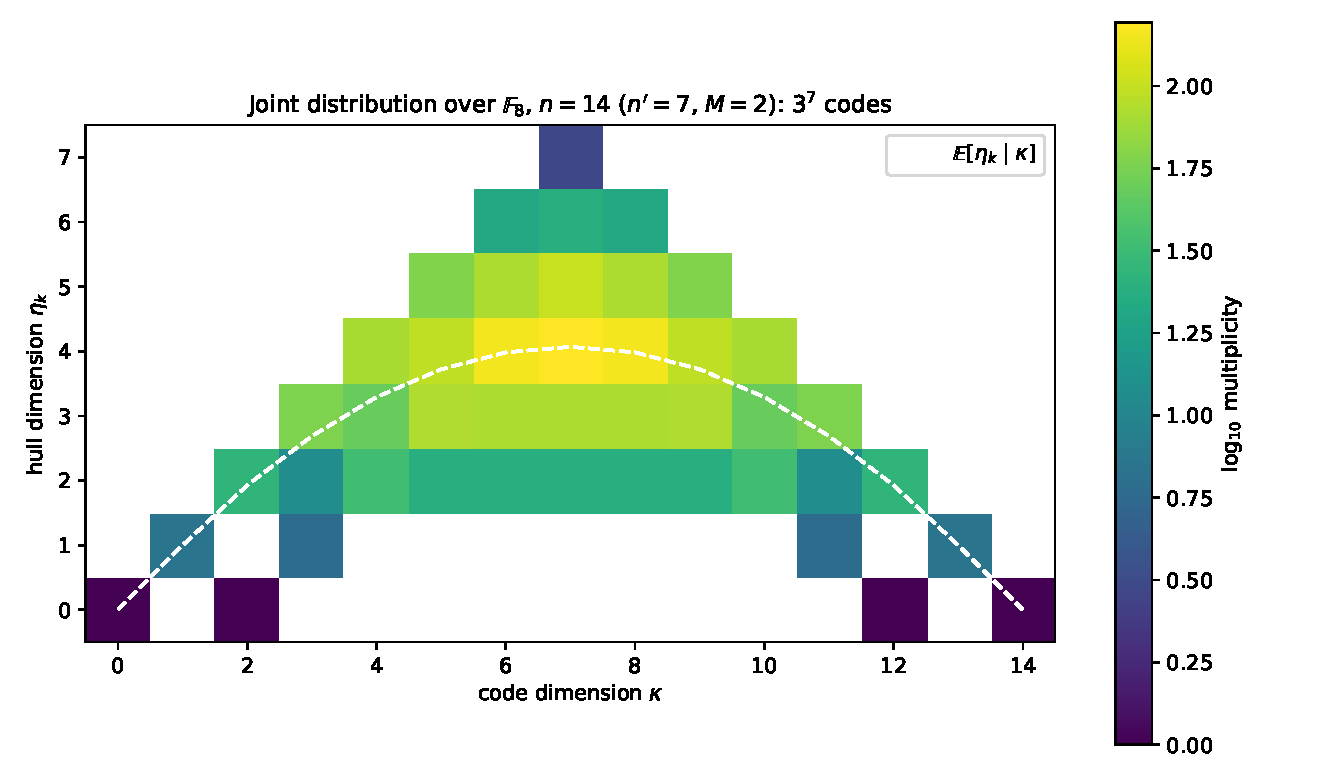
\includegraphics[width=0.82\linewidth]{fig2_joint_F8_n14.pdf}
\caption{Joint distribution $N_{\kappa,\eta}$ for $\F_8$, $n=14$
(Example~\ref{ex:F8}); color is $\log_{10}N_{\kappa,\eta}$ and white cells
are zero.  Only $\kappa\in\{1,3,11,13\}$ occur at $\eta=1$ --- the
one-orbit trapezoid gaps of Theorem~\ref{thm:support}, invisible from the
hull marginal alone.}
\label{fig:F8-joint}
\end{figure*}

\begin{example}\label{ex:mixed}
Let $\A=\F_4\times\F_{16}$ over $\F_4$, $n=10$ ($n'=5$, $M=2$),
$\lambda_0=\lambda=(1,1)$, $k=1$.  The $\F_4$ component contributes orbits
$(1,1),(2,2)$ as in Example~\ref{ex:F4}; the $\F_{16}$ component has
$m_s=[\F_{16}:\F_4]=2$ and contributes $(1,2),(4,2)$ --- the weight
$w_O=m_sd_O$ doubling in action.  Here $W=30$, there are $3^8=6561$ codes,
$123$ joint terms, $16$ LCD codes, $9$ self-dual codes, and
$\mathbb{E}[\eta_1]=23/3$, $\operatorname{Var}(\eta_1)=458/81$.  This family
is obtained from the $\F_4$ skeleton of Example~\ref{ex:F4} and the
$\F_{16}$ skeleton with the weights of Proposition~\ref{prop:global-selection}
doubled, and is reproduced by the enumerator (Table~\ref{tab:summary}).
\end{example}

\begin{example}\label{ex:char35}
Three families in odd characteristic illustrate the $a_O=1$ and $a_O=2$
phenomena of Sections~\ref{sec:short-orbits} and
\ref{sec:consequences}.
\begin{enumerate}
\item[\textup{(a)}] $K=\F_3$, $n=12$ ($n'=4$, $M=3$), $\lambda_0=\lambda=1$,
$k=0$: orbits $(1,1),(1,1),(1,2)$; $64$ codes, $33$ joint terms, $8$ LCD
codes, and \emph{no} self-dual code --- every orbit has odd length and $M$
is odd (Corollary~\ref{cor:self-dual}).
\item[\textup{(b)}] $K=\F_9=\F_3(i)$, $n=12$ ($n'=4$, $M=3$),
$\lambda_0=i$, $\lambda=-i$, $k=1$: a single orbit $(2,2)$, only $16$ codes
and $7$ joint terms.  By Proposition~\ref{prop:short-orbits}(ii) the hull
dimension is forced: $\eta=\min\{\kappa,12-\kappa\}$; there are $4$ self-dual
codes.
\item[\textup{(c)}] $K=\F_{25}$, $n=30$ ($n'=6$, $M=5$),
$\lambda_0=\lambda=1$, $k=1$: six fixed factors, orbits $(1,1)^6$; $46656$
codes, and all hull contribution comes from length-$1$ orbits through
$\min\{e,5-e\}$, with $\mathbb{E}[\eta_1]=6$ --- note the loop mean
$\nu_5=1$, not $\mu_5$ (Proposition~\ref{prop:moments}).
\end{enumerate}
\end{example}

\begin{example}\label{ex:F32}
Let $K=\F_{32}$, $n'=31$, $\lambda_0=\lambda=1$, $k=1$.  By
\eqref{eq:root-exponents} the reciprocal acts on the $31$ root exponents by
$j\mapsto-16j\bmod 31$, of order $10$ on the nonzero residues; hence the
orbit skeleton is $(1,1),(10,1),(10,1),(10,1)$ for every $M=2^t$.
\begin{itemize}
\item $M=2$, $n=62$: $3^{31}=617{,}673{,}396{,}283{,}947$ codes, $916$
nonzero joint coefficients, LCD $16$, self-orthogonal
$70{,}639{,}674{,}082$, self-dual $27$, $\mathbb{E}[\eta_1]=17$,
$\operatorname{Var}(\eta_1)=14/3$, and
$\max_\kappa\mathbb{E}[\eta_1\mid\kappa]\approx17.392$ at $\kappa=31$.
\item $M=4$, $n=124$ ($t=2$):
$5^{31}=4{,}656{,}612{,}873{,}077{,}392{,}578{,}125$ codes, $3531$ joint
coefficients, LCD still $16$, self-dual $125=5^3$,
$\mathbb{E}[\eta_1]=184/5$, $\operatorname{Var}(\eta_1)=326/25$.
\end{itemize}
In both cases the exact joint distribution over all $(M+1)^{31}$ codes is
obtained from the four orbit traces, with no enumeration of codes.
Figure~\ref{fig:F32-joint} shows the $M=2$ distribution.  For $M=2,4$,
the conditional means $\mathbb{E}[\eta_1\mid\kappa]$ peak at about $0.281\,W$ and
$0.302\,W$, in line with the $W/3$ regime of
Remark~\ref{rem:asymptotic-moments} (the skeleton limit is
$\frac{1/4+30/3}{31}\approx0.331$).
\end{example}

\begin{figure*}[!t]
\centering
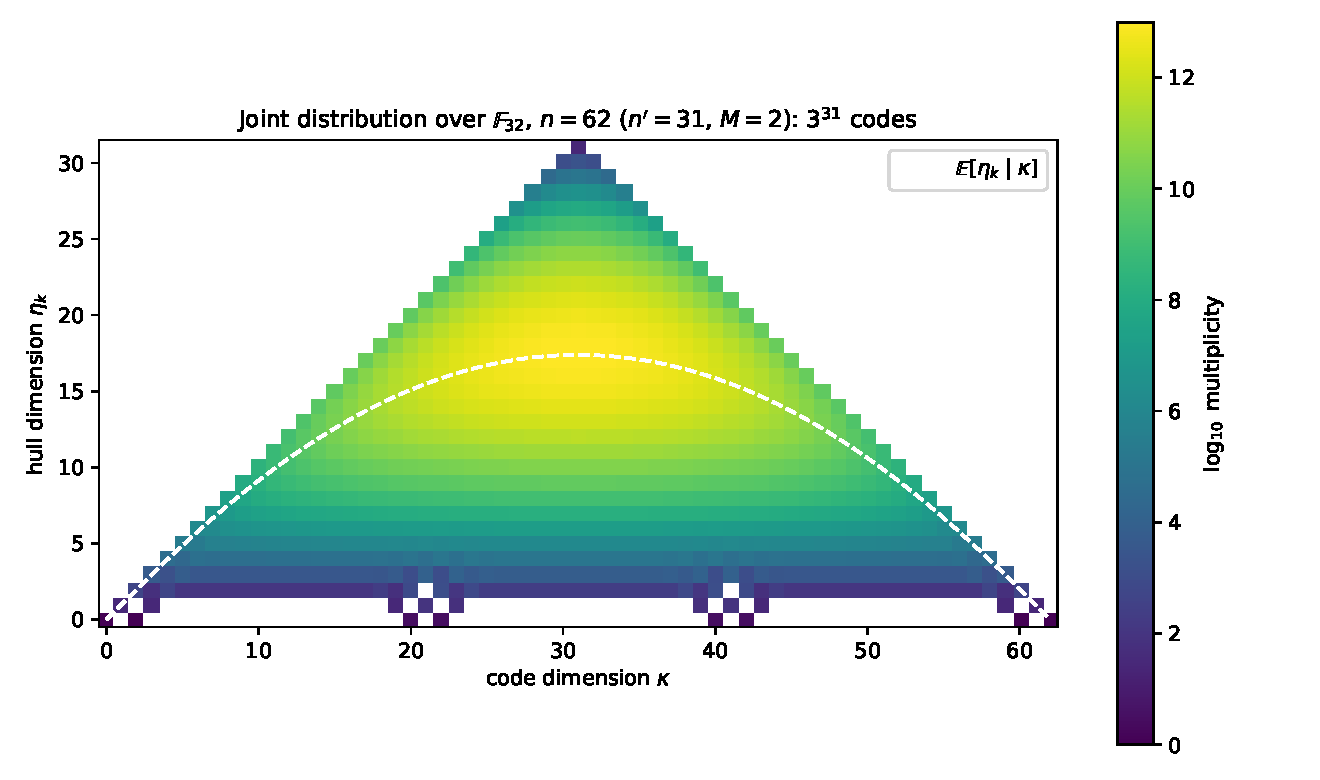
\includegraphics[width=0.82\linewidth]{fig3_joint_F32_n62.pdf}
\caption{Exact joint distribution for $\F_{32}$, $n=62$, $M=2$
(Example~\ref{ex:F32}), over all $3^{31}$ codes; color is
$\log_{10}N_{\kappa,\eta}$.  The periodic white holes at small $\eta$ are
the superposition of the three length-$10$ orbit trapezoids.}
\label{fig:F32-joint}
\end{figure*}

Table~\ref{tab:summary} collects all computed families; the full coefficient
lists are in the supplementary files \texttt{joint\_*.csv}.

\begin{table*}[!t]
\centering
\scriptsize
\setlength{\tabcolsep}{2.5pt}
\caption{Computed families (all with $\lambda=\lambda_0^M$; $k$ as shown).
Regenerated by \texttt{generate\_tables.py}; see
\texttt{summary\_families.csv}.}
\label{tab:summary}
\begin{tabular}{lcclrrrrcc}
\toprule
Family & $(n',M,n)$ & $k$ & orbits $(a_O,w_O)$ & codes & terms & LCD & SD &
$\mathbb{E}\eta_k$ & $\operatorname{Var}\eta_k$\\
\midrule
$\F_4$, $\lambda_0{=}1$ & $(5,2,10)$ & 1 & $(1,1),(2,2)$ & 27 & 15 & 4 & 3 & $23/9$ & $194/81$\\
$\F_4$, $\lambda_0{=}\omega$ & $(5,2,10)$ & 1 & $(1,1),(2,2)$ & 27 & 15 & 4 & 3 & $23/9$ & $194/81$\\
$\F_8$ & $(7,2,14)$ & 1 & $(1,1),(6,1)$ & 2187 & 44 & 4 & 3 & $11/3$ & $10/9$\\
$\F_3$ & $(4,3,12)$ & 0 & $(1,1)^2,(1,2)$ & 64 & 33 & 8 & 0 & $2$ & $3/2$\\
$\F_9$, $\lambda_0{=}i$ & $(4,3,12)$ & 1 & $(2,2)$ & 16 & 7 & 2 & 4 & $7/2$ & $15/4$\\
$\F_9$, $\lambda_0{=}-1$ & $(4,3,12)$ & 1 & $(2,1)^2$ & 256 & 22 & 4 & 16 & $7/2$ & $15/8$\\
$\F_9$ & $(8,3,24)$ & 1 & $(1,1)^4,(2,1)^2$ & 65536 & 142 & 64 & 0 & $11/2$ & $23/8$\\
$\F_{25}$ & $(6,5,30)$ & 1 & $(1,1)^6$ & 46656 & 191 & 64 & 0 & $6$ & $4$\\
$\F_4{\times}\F_{16}$ & $(5,2,10)$ & 1 & $(1,1),(2,2),(1,2),(4,2)$ & 6561 & 123 & 16 & 9 & $23/3$ & $458/81$\\
$\F_{32}$ & $(31,2,62)$ & 1 & $(1,1),(10,1)^3$ & $3^{31}$ & 916 & 16 & 27 & $17$ & $14/3$\\
$\F_{32}$ & $(31,4,124)$ & 1 & $(1,1),(10,1)^3$ & $5^{31}$ & 3531 & 16 & 125 & $184/5$ & $326/25$\\
\bottomrule
\end{tabular}
\end{table*}


\subsection{Independent verification}\label{sec:verification}

The computations are checked at two independent levels; both are reproduced
by the two scripts in \texttt{code/}, whose complete output is
\texttt{checks\_output.txt}.

\paragraph{Level 1: internal combinatorics.}  The script
\texttt{checks.py} compares the transfer-matrix trace with brute-force
enumeration of all exponent words for every $(a,M,w)$ with $a\leq6$, $M\leq5$
and $w\in\{1,2\}$ (60 cases); checks the closed forms of
Proposition~\ref{prop:short-orbits}; verifies the complement--reversal symmetry,
the checksum $\Epoly(1,1)=(M+1)^{N_F}$, the LCD count and the one-orbit
trapezoid of Theorem~\ref{thm:support} for $M\leq5$, $a\leq6$; verifies the
moment formulas of Proposition~\ref{prop:moments} for $M\leq7$ on a range of
skeletons; and recomputes every row of Table~\ref{tab:summary}, the joint table
of Example~\ref{ex:F4}, the conditional mean of Example~\ref{ex:F8} and the
maximal conditional mean of Example~\ref{ex:F32} from the enumerator alone.

\paragraph{Level 2: direct finite-field linear algebra.}  For the families of
Table~\ref{tab:verification} the script starts from the definitions, with no
orbit input: it factors $x^{n'}-\lambda_{s,0}$ over $K_s$ into distinct
irreducible factors, computes the reciprocal $f^{\#_{s,k}}$ from its definition
\eqref{eq:reciprocal}, and reads off the orbit skeleton, which is found to agree
with the skeletons used in Examples~\ref{ex:F4}--\ref{ex:char35}.  For
\emph{every} exponent word it then builds $g_{\mathbf{e}}=\prod f^{e_f}$, forms
the generator matrix $B$ from the $n-\deg g_{\mathbf{e}}$ non-wrapped shifts of
$g_{\mathbf{e}}$, and computes
\[
\eta_k=\dim C-\rank\bigl(B\,\sigma_{s,k}(B)^{\mathsf T}\bigr)
\]
over $K_s$ (Remark~\ref{rem:candidate}).  The resulting joint histogram is
compared with the trace product of Theorem~\ref{thm:main}; every word and every
histogram matches.  Characteristics $2$ and $3$, the Galois indices $k=0$ and
$k=1$, the multiplicities $M=2$ and $M=3$, and both fixed and swapped factors
are represented, so that the sign and normalization choices in $f^{\#_{s,k}}$
are exercised outside a single degenerate situation.  The larger families of
Table~\ref{tab:summary} ($\F_4\times\F_{16}$, $\F_{25}$, $\F_{32}$) are not
reached by this brute-force verification; for them the orbit data are read off
the factorization and only the transfer product is evaluated.

\begin{table*}[!t]
\centering
\scriptsize
\setlength{\tabcolsep}{2.5pt}
\caption{Direct finite-field verification coverage
(\texttt{checks\_output.txt}; in every row $\lambda=\lambda_0^M$ and the
alphabet is a single field).  ``Exhaustive'' means that the Gram-matrix rank
was computed for every exponent word and that the full joint histogram was
compared with the trace product of Theorem~\ref{thm:main}.}
\label{tab:verification}
\begin{tabular}{lrrrrlrr}
\toprule
Family & $p^m$ & $n'$ & $M$ & $n$ & $k$ & orbits & words checked\\
\midrule
$\F_4$, $\lambda_0=1$ & $2^2$ & 3 & 2 & 6  & 1 & $(1,1)^3$          & $3^3=27$\\
$\F_4$, $\lambda_0=1$ & $2^2$ & 5 & 2 & 10 & 1 & $(1,1),(2,2)$      & $3^3=27$\\
$\F_4$, $\lambda_0=\omega$ & $2^2$ & 5 & 2 & 10 & 1 & $(1,1),(2,2)$ & $3^3=27$\\
$\F_8$, $\lambda_0=1$ & $2^3$ & 7 & 2 & 14 & 1 & $(1,1),(6,1)$      & $3^7=2187$\\
$\F_3$, $\lambda_0=1$ & $3^1$ & 4 & 3 & 12 & 0 & $(1,1)^2,(1,2)$    & $4^3=64$\\
$\F_9$, $\lambda_0=i$ & $3^2$ & 4 & 3 & 12 & 1 & $(2,2)$            & $4^2=16$\\
$\F_9$, $\lambda_0=-1$ & $3^2$ & 4 & 3 & 12 & 1 & $(2,1)^2$         & $4^4=256$\\
\bottomrule
\end{tabular}
\end{table*}

\section{Conclusions}\label{sec:conclusions}
In this paper, we have determined the exact joint distribution of code dimension and
$k$-Galois hull dimension for all $\A$-linear $\lambda$-constacyclic codes
of arbitrary length over a square-free affine algebra. Writing each
repeated-root modulus as a power of its square-free kernel reduces a code to
an exponent selection; on each compatible reciprocal orbit the hull statistic
is a cyclic sum of pairwise minima and is encoded by a transfer-matrix trace,
while incompatible components contribute explicit dimension-only factors. The
resulting enumerator yields the marginal laws, exact one-orbit support,
means, variances and conditional laws, and the numbers of LCD,
self-orthogonal, dual-containing and self-dual codes. Given the orbit data,
its coefficients can be computed in time polynomial in $n$, $M$ and the
number of distinct kernel factors; the implementation has been checked by
direct finite-field linear algebra and evaluates, in particular, the
enumerator for all $3^{31}$ codes of length $62$ over $\F_{32}$. Throughout,
codes are counted as labeled $\A$-submodules, and no minimum-distance
assertion is made.

The scope of the result should be stated as plainly as its content. First, all
counts are over \emph{labeled} exponent selections: codes are not identified up
to monomial equivalence or isometry, so the enumerator describes the raw
population of $\A$-submodules rather than a set of equivalence classes.
Second, the formulas presuppose the orbit data of the reciprocal permutation
$\tau_{s,k}$ on $\Fs$; producing that data requires factoring the square-free
kernel $x^{n'}-\lambda_{s,0}$ over $K_s$, which is inexpensive for the lengths
treated here but is a genuine input rather than something the enumerator
supplies. Third, the parameter $M=p^t$ is common to all components because the
length $n$ is; different lengths over different components are not covered.
Fourth, nothing here concerns the minimum distance, the weight enumerator, or
the decoding problem, and no claim of optimality for the codes counted is made.

Beyond these limits, two directions seem most natural. One is the joint law of
the code dimension $\kappa$ together with the hull dimensions
$\eta_{k_1},\ldots,\eta_{k_r}$ for several Galois parameters
$k_1,\ldots,k_r$; such a multivariate enumerator would require a transfer-state
description that tracks the exponent relations arising from all the reciprocal
actions simultaneously, and it is not a consequence of the single-$k$ formula.
The other is the passage from labeled to unlabeled counts by combining the
transfer-matrix traces with a Burnside average over the monomial automorphism
group of the ambient algebra.


\section*{Acknowledgment}
All symbolic and numerical checks reported in the verification section were
carried out with the two Python scripts \texttt{enumerator.py} and
\texttt{checks.py} accompanying the manuscript; the saved output of the latter
reproduces every table and every example of the paper.
The authors used an AI-assisted writing tool (Arena.ai Agent Mode) to help
organize the literature, to edit the presentation, and to develop and check the
Python code used for the verification; all mathematical statements, proofs and
computed data were reviewed and verified by the authors, who take full
responsibility for the content of the article.

\bibliographystyle{IEEEtran}
\bibliography{references}

\end{document}
